\documentclass[11pt,a4paper]{article}

\usepackage[a4paper,left=2.2cm,right=2.2cm,top=2.4cm,bottom=2.4cm]{geometry}
\usepackage[T1]{fontenc}
\usepackage[utf8]{inputenc}
\usepackage{lmodern}
\usepackage{microtype}
\usepackage{graphicx}
\usepackage{booktabs}
\usepackage{tabularx}
\usepackage{longtable}
\usepackage{array}
\usepackage{float}
\usepackage{caption}
\usepackage{enumitem}
\usepackage{hyperref}
\usepackage{xcolor}
\usepackage{titlesec}
\usepackage{fancyhdr}
\usepackage{lastpage}
\usepackage{tcolorbox}
\usepackage{amsmath}
\usepackage{amssymb}
\usepackage{multirow}
\usepackage{colortbl}
\usepackage{tikz}
\usetikzlibrary{positioning,shapes.geometric}

\tcbuselibrary{skins,breakable}

\hypersetup{
  colorlinks=true,linkcolor=black,urlcolor=black,citecolor=black,
  pdftitle={PHOENIX Evaluation Study --- Phase 1 Generation Survey (HCP)},
  pdfauthor={Stijn Van Severen --- Ghent University}
}

% ── Colour palette ─────────────────────────────────────────────────────────
\definecolor{PrimaryBlue}{HTML}{1D4ED8}
\definecolor{DarkBlue}{HTML}{1E3A5F}
\definecolor{TealGreen}{HTML}{0E7490}
\definecolor{ForestGreen}{HTML}{047857}
\definecolor{GoldAmber}{HTML}{B45309}
\definecolor{RichPurple}{HTML}{6D28D9}
\definecolor{SlateMid}{HTML}{475569}
\definecolor{BorderGrey}{HTML}{CBD5E1}
\definecolor{SoftBG}{HTML}{F8FAFC}
\definecolor{AccentBlue}{HTML}{DBEAFE}
\definecolor{AccentGreen}{HTML}{D1FAE5}
\definecolor{AccentAmber}{HTML}{FEF3C7}
\definecolor{AccentPurple}{HTML}{EDE9FE}
\definecolor{AccentRed}{HTML}{FFE4E6}
\definecolor{AccentTeal}{HTML}{CFFAFE}
\definecolor{ComplaintBG}{HTML}{EFF6FF}
\definecolor{ContextBG}{HTML}{F0FDF4}
\definecolor{ResponseBG}{HTML}{FFFBEB}
\definecolor{PartOneBG}{HTML}{EFF6FF}
\definecolor{PartTwoBG}{HTML}{F0FDF4}
\definecolor{PartThreeBG}{HTML}{FFFBEB}
\definecolor{PartFourBG}{HTML}{FAF5FF}
\definecolor{PartFiveBG}{HTML}{FFF1F2}

% ── Typography ──────────────────────────────────────────────────────────────
\titleformat{\section}{\Large\bfseries\color{DarkBlue}}{\thesection}{0.7em}{}[\vspace{-0.2em}\color{PrimaryBlue}\rule{\textwidth}{0.6pt}]
\titleformat{\subsection}{\large\bfseries\color{PrimaryBlue}}{\thesubsection}{0.6em}{}
\titleformat{\subsubsection}{\normalsize\bfseries\color{TealGreen}}{\thesubsubsection}{0.5em}{}

\setlist[itemize]{topsep=3pt,itemsep=2pt,leftmargin=1.4em}
\setlist[enumerate]{topsep=3pt,itemsep=2pt,leftmargin=1.6em}
\setlength{\parskip}{0.45em}
\setlength{\parindent}{0pt}
\renewcommand{\arraystretch}{1.30}

% ── Page style ──────────────────────────────────────────────────────────────
\pagestyle{fancy}\fancyhf{}
\fancyhead[L]{\small\color{SlateMid}PHOENIX Evaluation Study --- Phase 1: Expert Generation}
\fancyhead[R]{\small\color{SlateMid}Healthcare Professional Survey}
\fancyfoot[C]{\small Page \thepage\ of \pageref{LastPage}}
\renewcommand{\headrulewidth}{0.3pt}\renewcommand{\footrulewidth}{0pt}

% ── Custom boxes ────────────────────────────────────────────────────────────
\newtcolorbox{complaintbox}[1][]{
  colback=ComplaintBG,colframe=PrimaryBlue,
  boxrule=0.8pt,arc=2.5mm,breakable,
  left=10pt,right=10pt,top=8pt,bottom=8pt,
  fonttitle=\small\bfseries\color{PrimaryBlue},
  title=Case Vignette,#1
}
\newtcolorbox{contextbox}[1][]{
  colback=ContextBG,colframe=ForestGreen,
  boxrule=0.6pt,arc=2mm,breakable,
  left=8pt,right=8pt,top=7pt,bottom=7pt,
  fonttitle=\small\bfseries\color{ForestGreen},
  title=Standardised Context from Prior Steps,#1
}
\newtcolorbox{responsebox}[1][]{
  colback=ResponseBG,colframe=GoldAmber,
  boxrule=0.7pt,arc=2mm,breakable,
  left=8pt,right=8pt,top=7pt,bottom=7pt,
  fonttitle=\small\bfseries\color{GoldAmber},
  title=Your Response,#1
}
\newtcolorbox{instrbox}[1][]{
  colback=SoftBG,colframe=BorderGrey,
  boxrule=0.5pt,arc=1.5mm,breakable,
  left=8pt,right=8pt,top=7pt,bottom=7pt,
  fonttitle=\bfseries\color{SlateMid},#1
}
\newtcolorbox{partbox}[2][]{
  colback=#2,colframe=DarkBlue,
  boxrule=1.0pt,arc=2.5mm,
  left=10pt,right=10pt,top=8pt,bottom=8pt,
  fonttitle=\large\bfseries\color{DarkBlue},
  title={#1}
}

% ── Helpers ─────────────────────────────────────────────────────────────────
\newcommand{\respline}{\vspace{0.3em}\noindent\rule{\textwidth}{0.3pt}}
\newcommand{\caseid}[1]{\noindent\textbf{\color{PrimaryBlue}Case #1}\quad}
\newcommand{\partlabel}[2]{\noindent{\large\bfseries\color{DarkBlue}Part #1 --- #2}\par\vspace{0.25em}}
\newcommand{\responsetextarea}[1]{\begin{tcolorbox}[colback=ResponseBG,colframe=GoldAmber,boxrule=0.6pt,arc=1.5mm,left=6pt,right=6pt,top=5pt,bottom=5pt]\small\textbf{\color{GoldAmber}Qualtrics item type:} Text Entry (Large / Essay). \quad \textit{Prompt:} #1\end{tcolorbox}}
\newcommand{\rankresponse}[1]{\begin{tcolorbox}[colback=ResponseBG,colframe=GoldAmber,boxrule=0.6pt,arc=1.5mm,left=6pt,right=6pt,top=5pt,bottom=5pt]\small\textbf{\color{GoldAmber}Qualtrics item type:} Rank Order. \quad \textit{Prompt:} #1\end{tcolorbox}}
\newcommand{\checkboxresponse}[1]{\begin{tcolorbox}[colback=ResponseBG,colframe=GoldAmber,boxrule=0.6pt,arc=1.5mm,left=6pt,right=6pt,top=5pt,bottom=5pt]\small\textbf{\color{GoldAmber}Qualtrics item type:} Multiple Choice (select all that apply) + optional Text Entry. \quad \textit{Prompt:} #1\end{tcolorbox}}
\newcommand{\dlnote}[1]{\par\vspace{0.15em}\noindent\begin{tcolorbox}[colback=AccentAmber,colframe=GoldAmber,boxrule=0.45pt,arc=1mm,left=5pt,right=5pt,top=2.5pt,bottom=2.5pt]\footnotesize\textbf{\color{GoldAmber}\scshape Qualtrics Display Logic:} Show this block only if participant code \textbf{=~#1}.\end{tcolorbox}\vspace{0.1em}}
\newcommand{\haparesponse}[1]{\begin{tcolorbox}[colback=ResponseBG,colframe=GoldAmber,boxrule=0.6pt,arc=1.5mm,left=6pt,right=6pt,top=5pt,bottom=5pt]\small\textbf{\color{GoldAmber}Qualtrics item type:} (A)~Multiple Choice --- HAPA phase; (B)~Text Entry (Medium) --- message. \quad \textit{Prompt:} #1\end{tcolorbox}}

% ── TikZ bipartite network styles ───────────────────────────────────────────
\tikzset{
  crnode/.style={draw=PrimaryBlue,fill=AccentBlue,rounded corners=2pt,
    minimum width=3.65cm,minimum height=0.50cm,
    font=\fontsize{6.5}{8}\selectfont\bfseries\color{PrimaryBlue},
    align=center,inner sep=2.5pt},
  prnode/.style={draw=TealGreen,fill=AccentTeal,rounded corners=2pt,
    minimum width=3.65cm,minimum height=0.50cm,
    font=\fontsize{6.5}{8}\selectfont\bfseries\color{TealGreen},
    align=center,inner sep=2.5pt},
  edgeS/.style={line width=1.6pt,draw=PrimaryBlue!75,opacity=0.80},
  edgeM/.style={line width=1.0pt,draw=TealGreen!80,opacity=0.75},
  edgeW/.style={line width=0.7pt,dashed,draw=gray!55,opacity=0.70},
}

\begin{document}

% ─────────────────────────────────────────────────────────────────────────────
%  COVER PAGE
% ─────────────────────────────────────────────────────────────────────────────
\begin{titlepage}
\centering\vspace*{0.8cm}

\begin{tcolorbox}[
  colback=DarkBlue,colframe=DarkBlue,
  arc=3mm,left=14pt,right=14pt,top=12pt,bottom=12pt,
  width=\textwidth
]
\centering
{\fontsize{22}{28}\selectfont\bfseries\color{white}
PHOENIX Evaluation Study\\[0.3em]
\fontsize{15}{20}\selectfont\color{AccentBlue}
Phase 1 --- Expert Generation Survey\\[0.2em]
\fontsize{12}{16}\selectfont\color{white}
\textit{Healthcare Professional (PRE) Instrument}
}
\end{tcolorbox}

\vspace{0.9cm}

\begin{tcolorbox}[
  colback=SoftBG,colframe=BorderGrey,
  arc=2mm,left=10pt,right=10pt,top=9pt,bottom=9pt,
  width=0.90\textwidth
]
\small\renewcommand{\arraystretch}{1.30}
\begin{tabularx}{\textwidth}{@{}>{\bfseries\raggedright}p{0.26\textwidth}X@{}}
Study title   & Evaluating the Clinical Quality of an Ontology-Based Multi-Agent Mental Health Support System (PHOENIX) \\
Institution   & Ghent University --- Faculty of Psychology and Educational Sciences \\
Researcher    & Stijn Van Severen (M.Sc.\ candidate) \\
Supervisors   & Prof.\ Geert Crombez; Dr.\ Annick De Paepe \\
Phase         & Phase 1 --- Generation (PRE) \\
Estimated time & Approximately 60 minutes (can be completed across multiple sessions) \\
Contact       & stijn.vanseveren@ugent.be \\
\end{tabularx}
\end{tcolorbox}

\vspace{0.7cm}

\begin{tcolorbox}[
  colback=AccentBlue,colframe=PrimaryBlue,
  arc=2mm,left=10pt,right=10pt,top=9pt,bottom=9pt,
  width=0.88\textwidth
]
\textbf{\color{PrimaryBlue}Thank you for participating.}

\medskip\small
You are taking part in a master's thesis evaluation study at Ghent University. The study examines a novel multi-agent artificial intelligence system --- called \textbf{PHOENIX} --- designed to support personalized digital mental health interventions. The system processes free-text complaints submitted by individuals experiencing mental health difficulties and works through a structured five-stage clinical reasoning process.

\medskip
This survey asks you to independently perform the \textbf{same five clinical reasoning tasks} on ten standardised case vignettes. Your responses will serve as the expert reference corpus in a subsequent double-blind evaluation (Phase 2) where independent healthcare professionals compare outputs from multiple sources without knowing their origin.

\medskip
There are no right or wrong answers. We are interested in your genuine clinical expertise and reasoning. Please respond as you would in an actual clinical context.
\end{tcolorbox}

\vfill

\begin{tcolorbox}[
  colback=SoftBG,colframe=BorderGrey,
  arc=1.5mm,left=8pt,right=8pt,top=7pt,bottom=7pt,
  width=0.82\textwidth
]
\centering\small
\textbf{This document is the survey blueprint for Qualtrics configuration.}\\
It contains the exact question text, case vignettes, standardised context, and response format specifications for all five parts of the Phase 1 survey.
\end{tcolorbox}

\vspace{0.4cm}{\large\today}
\end{titlepage}

\newpage
\tableofcontents
\newpage

% ─────────────────────────────────────────────────────────────────────────────
\section{Introduction and Participant Information}
% ─────────────────────────────────────────────────────────────────────────────

\subsection{Background: The PHOENIX System and Its Conceptual Framework}

PHOENIX (\textbf{P}ersonalized \textbf{H}ierarchical \textbf{O}ptimization \textbf{E}ngine for \textbf{N}avigating \textbf{I}nsightful e\textbf{X}plorations) is a multi-agent AI pipeline developed as part of a master's thesis in psychology at the Faculty of Psychology and Educational Sciences (FPPW) of Ghent University. The system is designed to support personalized longitudinal mental health interventions by processing a free-text complaint and producing a structured five-step clinical reasoning output.

PHOENIX is grounded in the \textbf{network theory of psychopathology} (Borsboom \& Cramer, 2013): mental health complaints are modelled not as expressions of a latent disorder, but as a \emph{dynamic network of interacting symptom components}. Two fundamental concepts underpin every step of the pipeline:

\begin{instrbox}[title=Key definitions: criterion vs.\ predictor]
\small
\textbf{Criterion (CR):} a clinically relevant, currently present \emph{symptom or complaint dimension} that can be repeatedly measured via daily EMA. Criteria are the \emph{outcome variables} of the network --- they describe \emph{what is going wrong} (e.g., sleep onset insomnia, panic episodes, depressed mood, guilt-based rumination). Criteria are \emph{not} behaviours, interventions, or causes.

\medskip
\textbf{Predictor (P):} a \emph{modifiable behavioural or process variable} that plausibly exerts a causal influence on one or more criteria and can be measured daily via a brief smartphone prompt. Predictors are the \emph{intervention variables} of the network --- they describe \emph{what can be changed} (e.g., evening screen time, planned exposure frequency, aerobic exercise, pre-sleep cognitive offloading). A predictor is \emph{never a symptom itself}, but a behaviour, strategy, or environmental factor that influences symptom levels.

\medskip\small
\textit{Clarifying examples:}
\begin{itemize}[topsep=1pt,itemsep=0pt]
\item \textbf{Criterion:} sleep onset insomnia, anticipatory anxiety, anergia, guilt-based rumination.
\item \textbf{Predictor:} evening screen time (min), planned exposure step (yes/no), aerobic exercise (min), pre-sleep offloading (yes/no).
\item \textbf{Neither criterion nor predictor:} appetite, resting heart rate, muscle tension --- these are state/symptom measures, not modifiable predictors.
\end{itemize}
\end{instrbox}

\medskip
The five stages of the PHOENIX pipeline mirror the core clinical reasoning tasks involved in formulation-driven digital intervention design:

\begin{center}
\renewcommand{\arraystretch}{1.40}
\small
\begin{tabular}{@{}>{\bfseries\color{PrimaryBlue}}p{0.07\textwidth}>{\bfseries}p{0.32\textwidth}p{0.50\textwidth}@{}}
\toprule
\textbf{Step} & \textbf{Clinical Task} & \textbf{System Output} \\
\midrule
01 & Operationalization of Mental State & List of 2--6 operationalized criterion variables derived from the complaint \\
02 & Initial Observational Model       & Bipartite network linking criteria to modifiable predictor variables \\
03 & Treatment-Target Identification   & Ranked shortlist of 2--4 modifiable treatment targets \\
04 & Updated Observational Model       & Refined measurement plan for the next monitoring cycle \\
05 & Tailored Intervention Message     & HAPA phase classification + 2--3 sentence coaching message \\
\bottomrule
\end{tabular}
\end{center}

\subsection{Your Role in This Study}

As a healthcare professional with relevant clinical expertise, you are asked to perform the same five clinical reasoning tasks independently and without reference to AI outputs. You will be assigned 	extbf{exactly two case vignettes} from the pool of ten (see Section~\ref{sec:assignment}). All five parts of this survey are completed for your two assigned cases only. Specifically, for each of your two assigned case vignettes:
\begin{itemize}
\item \textbf{Part 1:} Identify and operationalize the key mental health criteria present in the complaint.
\item \textbf{Part 2:} Propose a set of modifiable predictor variables that could be monitored over time.
\item \textbf{Part 3:} Identify and prioritize the most appropriate treatment targets.
\item \textbf{Part 4:} Refine the measurement plan for the next monitoring cycle.
\item \textbf{Part 5:} Write a brief, personalized digital coaching message.
\end{itemize}

Your responses will be compared to PHOENIX outputs in a double-blind evaluation. The comparing evaluators will not know which outputs came from a human expert and which from the AI system.

\subsection{Important Instructions}

\begin{instrbox}[title=Please read before beginning]
\begin{enumerate}
\item \textbf{Work independently.} Do not consult colleagues, clinical guidelines, or other resources while completing this survey. We are interested in your personal clinical knowledge and judgment.
\item \textbf{Use the standardised context.} Parts 2--5 provide you with context from previous steps. Please base your responses on this standardised context rather than generating your own prior-step outputs. This ensures all participants work from identical inputs.
\item \textbf{Be concise but specific.} There is no required minimum length. Short, precise responses are preferred over lengthy ones. Aim for clinical clarity.
\item \textbf{Use the case profiles.} Each vignette indicates the person's approximate age, occupation, and complaint duration. Use this background as you would in a brief referral letter.
\item \textbf{Work through the parts in order.} Parts are designed to build sequentially. You may complete the survey across multiple sessions but please complete each part in a single sitting if possible.
\item \textbf{If a case does not fit your primary discipline,} use your best clinical judgment based on your broader mental health knowledge.
\end{enumerate}
\end{instrbox}

\subsection{Ethical Notice}

Participation is voluntary. Your responses will be pseudonymized before analysis and will not be shared outside the research team. The data will be used exclusively for the purpose of this thesis evaluation study. You may withdraw at any time by contacting the researcher. By proceeding, you confirm that you have read this information sheet and consent to participate.

\subsection{Estimated Session Length}

\begin{center}
\small
\begin{tabular}{@{}>{\bfseries}p{0.06\textwidth}p{0.38\textwidth}p{0.20\textwidth}p{0.22\textwidth}p{0.04\textwidth}@{}}
\toprule
\textbf{Part} & \textbf{Task} & \textbf{Response format} & \textbf{Est.\ time} & \\
\midrule
1 & Operationalization     & Structured text (label + description)   & $\approx$6 min & \\
2 & Initial Obs.\ Model    & Structured text (predictor + edges)     & $\approx$6 min & \\
3 & Treatment Targets      & Rank-order with bipartite visual         & $\approx$7 min & \\
4 & Updated Obs.\ Model    & Checkbox selection + optional note       & $\approx$5 min & \\
5 & Intervention Message   & HAPA phase + 2--3 sentence message       & $\approx$8 min & \\
\midrule
  & \textbf{Total (2 cases)} & 10 structured items (2 cases $\times$ 5 parts) & \textbf{$\approx$30--40 min} & \\
\bottomrule
\end{tabular}
\end{center}

\newpage

\newpage

% ─────────────────────────────────────────────────────────────────────────────
\section{Case Assignment Protocol}
\label{sec:assignment}
% ─────────────────────────────────────────────────────────────────────────────

\begin{tcolorbox}[colback=AccentAmber,colframe=GoldAmber,arc=2.5mm,boxrule=1.0pt,left=10pt,right=10pt,top=9pt,bottom=9pt]
\textbf{\color{GoldAmber}Important: You only complete your two assigned cases.}

\medskip\small
This survey uses a \textbf{distributed assignment design}. The ten case vignettes are divided non-overlappingly across five healthcare professionals. You are assigned exactly two cases. This ensures all ten cases receive genuine independent expert responses, while keeping your total time to approximately 30--40 minutes.

Each participant's two responses are later pooled with the other HCPs' responses to form a corpus of ten unique expert outputs --- one per case --- which are then used in Phase~2 (POST evaluation).
\end{tcolorbox}

\vspace{0.6em}

\subsection*{HCP-to-Case Assignment Table}

\begin{center}
\renewcommand{\arraystretch}{1.45}
\small
\begin{tabular}{@{}>{\bfseries\color{PrimaryBlue}}p{0.14\textwidth}>{\bfseries}p{0.20\textwidth}p{0.52\textwidth}@{}}
\toprule
\textbf{Participant Code} & \textbf{Assigned Cases} & \textbf{Case Profiles} \\
\midrule
HCP-PRE-01 & C01 + C02 & 28-yr software developer (sleep/stress) \quad|\quad 34-yr admin (panic/avoidance) \\
HCP-PRE-02 & C03 + C04 & 41-yr teacher (burnout/withdrawal) \quad|\quad 63-yr retiree (grief/rumination) \\
HCP-PRE-03 & C05 + C06 & 25-yr student (OCD-type) \quad|\quad 32-yr marketing (performance anxiety) \\
HCP-PRE-04 & C07 + C08 & 46-yr manager (depression) \quad|\quad 38-yr project manager (ADHD) \\
HCP-PRE-05 & C09 + C10 & 27-yr sales rep (BPD-type) \quad|\quad 52-yr director (stress/alcohol coping) \\
\bottomrule
\end{tabular}
\end{center}

\vspace{0.5em}

\subsection*{Qualtrics Display Logic Implementation}

In the Qualtrics survey, a screening question at the beginning asks participants to select their assigned participant code from a dropdown (single-choice: HCP-PRE-01 through HCP-PRE-05). Each case block throughout all five parts is then set to \textbf{Display Logic: Show this block if Q\_ParticipantCode = [relevant code]}.

\begin{center}
\small\renewcommand{\arraystretch}{1.35}
\begin{tabular}{@{}>{\bfseries\color{TealGreen}}p{0.12\textwidth}p{0.35\textwidth}p{0.38\textwidth}@{}}
\toprule
\textbf{Qualtrics Block} & \textbf{Display Condition} & \textbf{Cases Shown} \\
\midrule
Block A & Q\_ParticipantCode = HCP-PRE-01 & C01 (all 5 parts) + C02 (all 5 parts) \\
Block B & Q\_ParticipantCode = HCP-PRE-02 & C03 (all 5 parts) + C04 (all 5 parts) \\
Block C & Q\_ParticipantCode = HCP-PRE-03 & C05 (all 5 parts) + C06 (all 5 parts) \\
Block D & Q\_ParticipantCode = HCP-PRE-04 & C07 (all 5 parts) + C08 (all 5 parts) \\
Block E & Q\_ParticipantCode = HCP-PRE-05 & C09 (all 5 parts) + C10 (all 5 parts) \\
\bottomrule
\end{tabular}
\end{center}

\vspace{0.3em}
\begin{instrbox}[title=Note for Qualtrics configurator]
\small For each of the five survey parts (Sections 4--8 of this document), the case items are grouped in pairs by assignment. Within each part, use Qualtrics Display Logic on the \emph{question block} level. The amber-bordered \textbf{Display Logic} annotation boxes throughout this document indicate the exact condition to apply to each case block.
\end{instrbox}


% ─────────────────────────────────────────────────────────────────────────────
\section{Case Vignettes Reference (All Parts)}
% ─────────────────────────────────────────────────────────────────────────────

The same ten cases are used throughout all five parts. This section provides the complete vignettes for reference. Each part will reproduce the relevant vignette alongside any additional standardised context.

\subsection*{Summary Reference Table}
\small
\begin{tabularx}{\textwidth}{@{}>{\bfseries\color{PrimaryBlue}}p{0.06\textwidth}>{\bfseries}p{0.28\textwidth}p{0.60\textwidth}@{}}
\toprule
\textbf{Case} & \textbf{Primary Presentation} & \textbf{Profile} \\
\midrule
C01 & Sleep onset insomnia + cognitive hyperarousal + social anhedonia + somatic tension & 28-year-old software developer; 2 months \\
C02 & Recurrent panic attacks + anticipatory anxiety + situational avoidance & 34-year-old healthcare administrator; 3 months \\
C03 & Professional burnout + emotional exhaustion + social withdrawal & 41-year-old secondary school teacher; 7 months \\
C04 & Complicated grief + insomnia + guilt-based rumination & 63-year-old retired professional; 9 months after loss \\
C05 & Intrusive harm-related thoughts + compulsive reviewing + avoidance & 25-year-old postgraduate student; 20 months \\
C06 & Professional performance anxiety + post-event rumination + advancement avoidance & 32-year-old marketing professional; $>$3 years \\
C07 & Persistent low mood + anergia + social isolation + hopelessness & 46-year-old accounts manager; 14 months \\
C08 & ADHD-related distress + executive dysfunction + relationship conflict & 38-year-old project manager; childhood onset \\
C09 & Emotional dysregulation + impulsivity + interpersonal instability & 27-year-old sales representative; 3 years \\
C10 & Chronic work stress + sleep maintenance insomnia + somatic + alcohol coping & 52-year-old operations director; 9 months \\
\bottomrule
\end{tabularx}

\newpage

% ─────────────────────────────────────────────────────────────────────────────
\section{Part 1: Operationalization of Mental State}
% ─────────────────────────────────────────────────────────────────────────────

\begin{tcolorbox}[colback=PartOneBG,colframe=PrimaryBlue,arc=2.5mm,boxrule=0.9pt,left=10pt,right=10pt,top=9pt,bottom=9pt]
\textbf{\color{PrimaryBlue}Part 1 Instructions}

\smallskip
\textbf{Task:} For each of your \textbf{two assigned case vignettes}, identify and operationalize the key mental health \textbf{criteria} present in the complaint. (This document shows all ten cases for researcher reference; Qualtrics Display Logic will show only your assigned two.)

\textbf{Definition --- Criterion (CR):} A criterion is a \textbf{distinct, currently present, clinically meaningful dimension of the person's symptom profile or functional impairment} that: (a) reflects a specific complaint aspect, (b) is a symptom or complaint \emph{state} (not a cause, behaviour, or demographic factor), and (c) can in principle be measured repeatedly over time via daily self-report.

\begin{itemize}[topsep=3pt,itemsep=2pt]
\item \textbf{Examples of valid criteria:} sleep onset insomnia, cognitive hyperarousal at bedtime, situational avoidance, recurrent intrusive thoughts, social anhedonia, post-event rumination, persistent depressed mood.
\item \textbf{Not criteria:} behavioural choices (``evening screen use''), presumed causes (``work stress''), physiological values (``resting heart rate''), or coping patterns (``alcohol use to relax'').
\end{itemize}

\textbf{Response format:} For each case, list \textbf{2--6 criteria}. For each criterion provide:
\begin{itemize}
\item A \textbf{short label} (2--5 words, e.g., ``Sleep onset insomnia'')
\item A \textbf{brief description} (1--2 sentences: what it is and how it manifests in this case)
\end{itemize}
Use the structured template: \texttt{Label | Description} on one line per criterion. This allows direct automated comparison with machine outputs.

\textbf{Qualtrics setup:} 2 open-text questions per HCP (Text Entry --- Large), shown via Display Logic. Prompt shown in each response box.

\textbf{Time:} Approximately 3 minutes per case ($\approx$6 minutes for your two cases).
\end{tcolorbox}

\vspace{0.5em}

% ── C01 ─────────────────────────────────────────────────────────────────────
\subsubsection*{Case C01}
\dlnote{HCP-PRE-01}

\begin{complaintbox}[title=Case C01 --- Complaint Vignette]
\textbf{Profile:} 28-year-old software developer; complaint duration: 2 months.

\smallskip
``Over the past two months I have been finding it very hard to fall asleep at night. My mind keeps going over everything I still need to do --- deadlines, unfinished tasks, conversations I need to have. Even when I am exhausted, I cannot seem to switch my thoughts off. Something else I have noticed is that I no longer enjoy social occasions the way I used to. I go to gatherings with friends and I feel disconnected, like I am watching everyone else have fun from a distance. My neck and shoulders are also constantly tense and sore, which my GP says is likely stress-related.''
\end{complaintbox}

\responsetextarea{Please list 2--6 operationalized criteria for this complaint. For each criterion, provide: (1) a short label (2--5 words) and (2) a brief description (1--2 sentences).}

\vspace{0.4em}
% ── C02 ─────────────────────────────────────────────────────────────────────
\subsubsection*{Case C02}
\dlnote{HCP-PRE-01}

\begin{complaintbox}[title=Case C02 --- Complaint Vignette]
\textbf{Profile:} 34-year-old healthcare administrator; complaint duration: 3 months.

\smallskip
``Around three months ago I started having episodes where my heart would pound, I felt like I could not get enough air, and I was convinced something terrible was happening to me. These episodes are frightening and can come out of nowhere, even when I am sitting quietly at home. Since they started, I have become scared of having one in public and have been avoiding supermarkets, public transport, and crowded places. I have called in sick to work several times because I was afraid of having an episode there. I know logically that these situations are not dangerous but I cannot stop the fear.''
\end{complaintbox}

\responsetextarea{Please list 2--6 operationalized criteria for this complaint. For each criterion, provide: (1) a short label (2--5 words) and (2) a brief description (1--2 sentences).}

\vspace{0.4em}
% ── C03 ─────────────────────────────────────────────────────────────────────
\subsubsection*{Case C03}
\dlnote{HCP-PRE-02}

\begin{complaintbox}[title=Case C03 --- Complaint Vignette]
\textbf{Profile:} 41-year-old secondary school teacher; complaint duration: 7 months.

\smallskip
``I have been teaching for fifteen years and I used to love my work, but over the past several months I feel completely empty. I go to school, deliver my lessons, and come home, but there is nothing left in me. I sit in front of the television every evening and cannot motivate myself to do anything else. I have stopped going out with friends and rarely reply to messages anymore. I have also started making mistakes at work --- forgetting things, losing track of where I am in a lesson --- which has never happened before. I feel ashamed about it but I do not know how to change things.''
\end{complaintbox}

\responsetextarea{Please list 2--6 operationalized criteria for this complaint. For each criterion, provide: (1) a short label (2--5 words) and (2) a brief description (1--2 sentences).}

\vspace{0.4em}
% ── C04 ─────────────────────────────────────────────────────────────────────
\subsubsection*{Case C04}
\dlnote{HCP-PRE-02}

\begin{complaintbox}[title=Case C04 --- Complaint Vignette]
\textbf{Profile:} 63-year-old retired professional; 9 months after bereavement.

\smallskip
``My partner died nine months ago and I am still not coping well. I think about them constantly. Random things --- a song, a smell, a television programme we used to watch together --- trigger intense waves of grief that I cannot control. I am not sleeping properly; I wake in the early hours and cannot get back to sleep. I also feel a lot of guilt. I keep going over things I said or should have said, and times I was not patient enough. I cannot imagine what my future is supposed to look like anymore. My family tells me I should be feeling better by now, but I am not.''
\end{complaintbox}

\responsetextarea{Please list 2--6 operationalized criteria for this complaint. For each criterion, provide: (1) a short label (2--5 words) and (2) a brief description (1--2 sentences).}

\vspace{0.4em}
% ── C05 ─────────────────────────────────────────────────────────────────────
\subsubsection*{Case C05}
\dlnote{HCP-PRE-03}

\begin{complaintbox}[title=Case C05 --- Complaint Vignette]
\textbf{Profile:} 25-year-old postgraduate student; complaint duration: approximately 20 months.

\smallskip
``I have thoughts that I might accidentally hurt people, even though I have no desire to do so and I know these thoughts are irrational. They come suddenly and feel very realistic and disturbing. After having one of these thoughts I spend a lot of time mentally reviewing what happened to reassure myself I have not done anything wrong. I have also started avoiding situations where I might hold something sharp, which affects my daily life and some social situations. This reviewing takes up hours of my day and is affecting my studies and my relationships.''
\end{complaintbox}

\responsetextarea{Please list 2--6 operationalized criteria for this complaint. For each criterion, provide: (1) a short label (2--5 words) and (2) a brief description (1--2 sentences).}

\vspace{0.4em}
% ── C06 ─────────────────────────────────────────────────────────────────────
\subsubsection*{Case C06}
\dlnote{HCP-PRE-03}

\begin{complaintbox}[title=Case C06 --- Complaint Vignette]
\textbf{Profile:} 32-year-old marketing professional; complaint persistent since early career ($>$3 years).

\smallskip
``I have a great deal of anxiety around professional situations. Whenever I have to give a presentation, speak in a meeting, or receive feedback from my manager, I become so self-conscious that my mind goes blank. I spend hours preparing what to say beforehand but then freeze in the moment anyway. Afterwards I replay everything that happened and analyse every word I said for a long time. I have turned down several promotions and interesting projects because I was afraid of the visibility they would bring. I know my anxiety about how others perceive me is disproportionate but I cannot seem to stop it.''
\end{complaintbox}

\responsetextarea{Please list 2--6 operationalized criteria for this complaint. For each criterion, provide: (1) a short label (2--5 words) and (2) a brief description (1--2 sentences).}

\vspace{0.4em}
% ── C07 ─────────────────────────────────────────────────────────────────────
\subsubsection*{Case C07}
\dlnote{HCP-PRE-04}

\begin{complaintbox}[title=Case C07 --- Complaint Vignette]
\textbf{Profile:} 46-year-old accounts manager; complaint duration: 14 months.

\smallskip
``For over a year I have woken up most mornings feeling heavy and grey. I would not call it dramatic sadness --- more like a persistent flatness where nothing feels worthwhile. Very simple tasks feel like enormous effort: getting dressed, replying to an email, cooking a meal. I have gradually lost touch with almost everyone I used to socialise with because I do not have the energy to maintain relationships. I sleep a lot but never feel rested. Privately I wonder whether I will ever feel like my old self again. I am seeking help because my GP told me I should.''
\end{complaintbox}

\responsetextarea{Please list 2--6 operationalized criteria for this complaint. For each criterion, provide: (1) a short label (2--5 words) and (2) a brief description (1--2 sentences).}

\vspace{0.4em}
% ── C08 ─────────────────────────────────────────────────────────────────────
\subsubsection*{Case C08}
\dlnote{HCP-PRE-04}

\begin{complaintbox}[title=Case C08 --- Complaint Vignette]
\textbf{Profile:} 38-year-old project manager; difficulties since childhood, significantly worsened over past 12 months.

\smallskip
``I have always struggled to concentrate on tasks that do not immediately interest me, but it has gotten much worse over the past year. I start projects and rarely finish them. I forget appointments even when I have written them down. My partner is frustrated with me because they say I do not listen and that I am unreliable. I am competent in many ways but I feel like a constant failure. I have started avoiding tasks I know I will struggle with, which makes the backlog worse. I feel ashamed that something that seems straightforward for other people is so hard for me.''
\end{complaintbox}

\responsetextarea{Please list 2--6 operationalized criteria for this complaint. For each criterion, provide: (1) a short label (2--5 words) and (2) a brief description (1--2 sentences).}

\vspace{0.4em}
% ── C09 ─────────────────────────────────────────────────────────────────────
\subsubsection*{Case C09}
\dlnote{HCP-PRE-05}

\begin{complaintbox}[title=Case C09 --- Complaint Vignette]
\textbf{Profile:} 27-year-old sales representative; complaint duration: 3 years.

\smallskip
``My mood changes very rapidly throughout the day and it often does not seem connected to what is actually happening around me. I can feel reasonably okay in the morning and be in tears by early afternoon. When I feel criticized or rejected, even over small things, my reaction is very intense --- I become angry or very distressed almost instantly. I also act impulsively, particularly with money or in relationships, and I regret it afterwards. My relationships tend to become intense very quickly but then fall apart. I am aware that this pattern repeats but I do not know how to break it.''
\end{complaintbox}

\responsetextarea{Please list 2--6 operationalized criteria for this complaint. For each criterion, provide: (1) a short label (2--5 words) and (2) a brief description (1--2 sentences).}

\vspace{0.4em}
% ── C10 ─────────────────────────────────────────────────────────────────────
\subsubsection*{Case C10}
\dlnote{HCP-PRE-05}

\begin{complaintbox}[title=Case C10 --- Complaint Vignette]
\textbf{Profile:} 52-year-old operations director; complaint duration: approximately 9 months.

\smallskip
``Work stress has been building for the better part of a year. I have constant tension headaches and my stomach is unsettled most days. I lie awake at night going over work problems and decisions that need to be made, and I rarely fall back to sleep after waking. I have been having two or three glasses of wine each evening to help me wind down, which I know is not ideal but it feels necessary. My exercise routine has completely stopped and I have put on weight. I snap at people at home and then feel guilty about it. I am holding everything together externally but I am running on empty.''
\end{complaintbox}

\responsetextarea{Please list 2--6 operationalized criteria for this complaint. For each criterion, provide: (1) a short label (2--5 words) and (2) a brief description (1--2 sentences).}

\newpage

% ─────────────────────────────────────────────────────────────────────────────
\section{Part 2: Initial Observational Model Construction}
% ─────────────────────────────────────────────────────────────────────────────

\begin{tcolorbox}[colback=PartTwoBG,colframe=ForestGreen,arc=2.5mm,boxrule=0.9pt,left=10pt,right=10pt,top=9pt,bottom=9pt]
\textbf{\color{ForestGreen}Part 2 Instructions}

\smallskip
\textbf{Task:} For each case, propose a set of \textbf{modifiable predictor variables} (P-nodes) that could be monitored via daily Ecological Momentary Assessment (EMA) to explain or predict the criteria identified in Part 1.

\textbf{Definition --- Predictor (P):} A predictor is a \textbf{modifiable behavioural or process variable} that: (a) can plausibly change the severity of one or more criteria, (b) can be measured by the person themselves with a simple daily rating, count, or yes/no, and (c) is itself a \emph{treatment option} --- not a symptom or an outcome.

\begin{itemize}[topsep=3pt,itemsep=2pt]
\item \textbf{Examples of valid predictors:} evening screen time (min), planned exposure attempts (yes/no), aerobic exercise session (min), pre-sleep cognitive offloading (yes/no), safety behaviour count (n).
\item \textbf{Not predictors:} symptom dimensions (``appetite today 0--10'', ``muscle tension 0--10''), diagnostic labels, or static background factors. These are criteria or confounders, not intervention levers.
\end{itemize}

\textbf{EMA principles:} Each predictor must be (1) \emph{daily-reportable} (takes $<$30 seconds to rate), (2) \emph{dynamic} (can vary from day to day), (3) \emph{operationally defined} (specific enough to measure unambiguously), and (4) \emph{clinically plausible} as a causal influence on at least one criterion.

The resulting predictor--criterion pairs form the edges of the \textbf{initial bipartite observational network} (Part 2), from which treatment targets are subsequently identified (Part 3).

\textbf{Response format:} List \textbf{3--6 predictors} using this structured template (one per line):

\begin{center}\small\ttfamily
Label | 1-sentence measurement definition | CR connections (e.g.\ CR-1, CR-3)
\end{center}

\textbf{Context provided:} Standardised criteria (from Step 01 reference run) appear for each case.

\textbf{Qualtrics setup:} 10 Text Entry (Large) questions. Copy the exact prompt shown in each response box.

\textbf{Time:} Approximately 3 minutes per case ($\approx$6 minutes for your two cases).
\end{tcolorbox}

\vspace{0.5em}

% ── C01 Part 2 ───────────────────────────────────────────────────────────────
\subsubsection*{Case C01 --- Part 2}
\dlnote{HCP-PRE-01}

\begin{complaintbox}[title=Case C01 --- Complaint (abbreviated)]
\small 28-year-old software developer, 2 months. Difficulty falling asleep; bedtime rumination about tasks and deadlines; social disconnection and reduced positive affect; constant neck and shoulder tension.
\end{complaintbox}

\begin{contextbox}
\small\textbf{Standardised criteria (from Step 01 reference run):}
\begin{itemize}[topsep=2pt,itemsep=1pt]
\item \textbf{CR-1} \textit{Sleep onset insomnia} --- subjective difficulty initiating sleep; estimated latency $>$30 min most nights.
\item \textbf{CR-2} \textit{Cognitive hyperarousal at bedtime} --- repetitive uncontrollable task-anticipatory thoughts at sleep onset.
\item \textbf{CR-3} \textit{Social anhedonia} --- reduced capacity to experience positive affect in social contexts.
\item \textbf{CR-4} \textit{Musculoskeletal stress tension} --- chronic neck and shoulder tension of probable stress etiology.
\end{itemize}
\end{contextbox}

\responsetextarea{Please propose 3--6 modifiable predictor variables for this case. For each predictor, provide: (1) short label, (2) brief measurement definition (1 sentence), (3) which criteria (CR-1 to CR-4) it connects to.}

\vspace{0.4em}

% ── C02 Part 2 ───────────────────────────────────────────────────────────────
\subsubsection*{Case C02 --- Part 2}
\dlnote{HCP-PRE-01}

\begin{complaintbox}[title=Case C02 --- Complaint (abbreviated)]
\small 34-year-old healthcare administrator, 3 months. Recurrent panic episodes (palpitations, breathlessness, impending-doom cognition); persistent fear of future episodes; avoidance of public settings; occupational impact.
\end{complaintbox}

\begin{contextbox}
\small\textbf{Standardised criteria (from Step 01 reference run):}
\begin{itemize}[topsep=2pt,itemsep=1pt]
\item \textbf{CR-1} \textit{Recurrent panic episodes} --- discrete episodes with autonomic arousal and sudden onset.
\item \textbf{CR-2} \textit{Anticipatory anxiety} --- persistent fear of having a further episode; interoceptive vigilance.
\item \textbf{CR-3} \textit{Situational avoidance} --- active avoidance of supermarkets, public transport, crowded venues.
\item \textbf{CR-4} \textit{Occupational interference} --- sick leave, avoidance of work attendance, reduced function.
\end{itemize}
\end{contextbox}

\responsetextarea{Please propose 3--6 modifiable predictor variables for this case. For each predictor: (1) short label, (2) measurement definition, (3) connected criteria.}

\vspace{0.4em}

% ── C03 Part 2 ───────────────────────────────────────────────────────────────
\subsubsection*{Case C03 --- Part 2}
\dlnote{HCP-PRE-02}

\begin{complaintbox}[title=Case C03 --- Complaint (abbreviated)]
\small 41-year-old teacher, 7 months. Emotional exhaustion; depersonalization/professional detachment; social withdrawal; concentration difficulties and occupational errors.
\end{complaintbox}

\begin{contextbox}
\small\textbf{Standardised criteria:}
\begin{itemize}[topsep=2pt,itemsep=1pt]
\item \textbf{CR-1} \textit{Emotional exhaustion} --- depleted affective resources; absence of professional engagement or motivation.
\item \textbf{CR-2} \textit{Professional depersonalization} --- detached, going-through-the-motions quality of occupational performance.
\item \textbf{CR-3} \textit{Social withdrawal} --- discontinued social activities; non-response to social contact.
\item \textbf{CR-4} \textit{Occupational cognitive impairment} --- concentration difficulties, memory failures, and increased error rate at work.
\end{itemize}
\end{contextbox}

\responsetextarea{Please propose 3--6 modifiable predictor variables for this case. For each predictor: (1) short label, (2) measurement definition, (3) connected criteria.}

\vspace{0.4em}

% ── C04 Part 2 ───────────────────────────────────────────────────────────────
\subsubsection*{Case C04 --- Part 2}
\dlnote{HCP-PRE-02}

\begin{complaintbox}[title=Case C04 --- Complaint (abbreviated)]
\small 63-year-old retired professional, 9 months post-bereavement. Prolonged grief with intrusive memories; sleep maintenance insomnia; guilt-based counterfactual rumination; inability to envision a future.
\end{complaintbox}

\begin{contextbox}
\small\textbf{Standardised criteria:}
\begin{itemize}[topsep=2pt,itemsep=1pt]
\item \textbf{CR-1} \textit{Prolonged grief response} --- intrusive memories, yearning, difficulty accepting the loss.
\item \textbf{CR-2} \textit{Sleep maintenance insomnia} --- early-morning awakening; inability to return to sleep.
\item \textbf{CR-3} \textit{Guilt-based counterfactual rumination} --- repetitive thoughts about past interactions; self-blame and regret.
\item \textbf{CR-4} \textit{Reduced future orientation} --- inability to imagine meaningful activities or goals beyond the loss.
\end{itemize}
\end{contextbox}

\responsetextarea{Please propose 3--6 modifiable predictor variables for this case. For each predictor: (1) short label, (2) measurement definition, (3) connected criteria.}

\vspace{0.4em}

% ── C05 Part 2 ───────────────────────────────────────────────────────────────
\subsubsection*{Case C05 --- Part 2}
\dlnote{HCP-PRE-03}

\begin{complaintbox}[title=Case C05 --- Complaint (abbreviated)]
\small 25-year-old postgraduate student, $\sim$20 months. Intrusive harm-related obsessional thoughts; compulsive mental reviewing; situational avoidance; significant daily time interference ($>$2 hours).
\end{complaintbox}

\begin{contextbox}
\small\textbf{Standardised criteria:}
\begin{itemize}[topsep=2pt,itemsep=1pt]
\item \textbf{CR-1} \textit{Intrusive harm-related obsessions} --- unwanted ego-dystonic thoughts of accidentally harming others.
\item \textbf{CR-2} \textit{Compulsive reviewing behavior} --- mental replaying and checking sequences triggered by intrusions.
\item \textbf{CR-3} \textit{Harm-trigger situational avoidance} --- avoidance of sharp objects, specific locations, and social settings.
\item \textbf{CR-4} \textit{OCD time interference} --- rituals and reviewing consuming $>$2 hours of productive daily time.
\end{itemize}
\end{contextbox}

\responsetextarea{Please propose 3--6 modifiable predictor variables for this case. For each predictor: (1) short label, (2) measurement definition, (3) connected criteria.}

\vspace{0.4em}

% ── C06 Part 2 ───────────────────────────────────────────────────────────────
\subsubsection*{Case C06 --- Part 2}
\dlnote{HCP-PRE-03}

\begin{complaintbox}[title=Case C06 --- Complaint (abbreviated)]
\small 32-year-old marketing professional, $>$3 years. Performance anxiety in professional situations; post-event rumination; pre-event preparation burden; avoidance of advancement opportunities.
\end{complaintbox}

\begin{contextbox}
\small\textbf{Standardised criteria:}
\begin{itemize}[topsep=2pt,itemsep=1pt]
\item \textbf{CR-1} \textit{Professional performance anxiety} --- fear and physiological arousal in presentations, meetings, and evaluations.
\item \textbf{CR-2} \textit{Post-event rumination} --- prolonged post-hoc analysis of social and professional performances.
\item \textbf{CR-3} \textit{Pre-event cognitive preparation burden} --- extensive anticipatory rehearsal consuming significant time and energy.
\item \textbf{CR-4} \textit{Advancement avoidance} --- declining opportunities due to anxiety about increased visibility.
\end{itemize}
\end{contextbox}

\responsetextarea{Please propose 3--6 modifiable predictor variables for this case. For each predictor: (1) short label, (2) measurement definition, (3) connected criteria.}

\vspace{0.4em}

% ── C07 Part 2 ───────────────────────────────────────────────────────────────
\subsubsection*{Case C07 --- Part 2}
\dlnote{HCP-PRE-04}

\begin{complaintbox}[title=Case C07 --- Complaint (abbreviated)]
\small 46-year-old accounts manager, 14 months. Persistent low mood and anhedonia; significant anergia; social isolation; hopelessness about recovery.
\end{complaintbox}

\begin{contextbox}
\small\textbf{Standardised criteria:}
\begin{itemize}[topsep=2pt,itemsep=1pt]
\item \textbf{CR-1} \textit{Persistent depressed mood} --- pervasive low mood and flatness most days for $>$12 months.
\item \textbf{CR-2} \textit{Anergia and psychomotor slowing} --- fatigue and effortful quality of routine daily tasks.
\item \textbf{CR-3} \textit{Social isolation} --- loss of social network through withdrawal and failure to maintain contact.
\item \textbf{CR-4} \textit{Hopelessness about recovery} --- stable negative expectation about future mood improvement.
\end{itemize}
\end{contextbox}

\responsetextarea{Please propose 3--6 modifiable predictor variables for this case. For each predictor: (1) short label, (2) measurement definition, (3) connected criteria.}

\vspace{0.4em}

% ── C08 Part 2 ───────────────────────────────────────────────────────────────
\subsubsection*{Case C08 --- Part 2}
\dlnote{HCP-PRE-04}

\begin{complaintbox}[title=Case C08 --- Complaint (abbreviated)]
\small 38-year-old project manager, childhood onset (worsened past 12 months). Sustained attention deficit; planning/organization failures; interpersonal inattentiveness; chronic performance shame.
\end{complaintbox}

\begin{contextbox}
\small\textbf{Standardised criteria:}
\begin{itemize}[topsep=2pt,itemsep=1pt]
\item \textbf{CR-1} \textit{Sustained attention deficit} --- difficulty maintaining focus on non-preferred, effortful tasks.
\item \textbf{CR-2} \textit{Planning and organization failures} --- missed appointments, incomplete tasks, failure to use organizational systems.
\item \textbf{CR-3} \textit{Interpersonal inattentiveness} --- partner reports not being listened to; perceived unreliability in relationships.
\item \textbf{CR-4} \textit{Chronic performance shame} --- pervasive self-judgment tied to executive functioning difficulties.
\end{itemize}
\end{contextbox}

\responsetextarea{Please propose 3--6 modifiable predictor variables for this case. For each predictor: (1) short label, (2) measurement definition, (3) connected criteria.}

\vspace{0.4em}

% ── C09 Part 2 ───────────────────────────────────────────────────────────────
\subsubsection*{Case C09 --- Part 2}
\dlnote{HCP-PRE-05}

\begin{complaintbox}[title=Case C09 --- Complaint (abbreviated)]
\small 27-year-old sales representative, 3 years. Rapid intra-day mood swings; intense emotional reactivity to perceived criticism/rejection; impulsive behaviour; recurrent relationship instability.
\end{complaintbox}

\begin{contextbox}
\small\textbf{Standardised criteria:}
\begin{itemize}[topsep=2pt,itemsep=1pt]
\item \textbf{CR-1} \textit{Rapid intra-day mood cycling} --- multiple significant mood shifts within a single day.
\item \textbf{CR-2} \textit{Emotional reactivity to rejection cues} --- intense and rapid affective response to perceived criticism or abandonment.
\item \textbf{CR-3} \textit{Impulsive behaviour patterns} --- poorly modulated spending, relationship decisions, or interpersonal actions.
\item \textbf{CR-4} \textit{Recurrent relationship instability} --- pattern of rapid escalation followed by breakdown in close relationships.
\end{itemize}
\end{contextbox}

\responsetextarea{Please propose 3--6 modifiable predictor variables for this case. For each predictor: (1) short label, (2) measurement definition, (3) connected criteria.}

\vspace{0.4em}

% ── C10 Part 2 ───────────────────────────────────────────────────────────────
\subsubsection*{Case C10 --- Part 2}
\dlnote{HCP-PRE-05}

\begin{complaintbox}[title=Case C10 --- Complaint (abbreviated)]
\small 52-year-old operations director, 9 months. Chronic occupational stress response; sleep maintenance insomnia; somatic stress symptoms; evening alcohol use as coping mechanism.
\end{complaintbox}

\begin{contextbox}
\small\textbf{Standardised criteria:}
\begin{itemize}[topsep=2pt,itemsep=1pt]
\item \textbf{CR-1} \textit{Chronic occupational stress} --- persistent physiological stress response driven by work demands.
\item \textbf{CR-2} \textit{Sleep maintenance insomnia} --- early awakening with prolonged wakefulness; ruminative nocturnal cognition.
\item \textbf{CR-3} \textit{Somatic stress expression} --- recurrent tension headaches and gastrointestinal symptoms.
\item \textbf{CR-4} \textit{Alcohol use as coping} --- regular evening alcohol consumption as a relaxation/sleep aid.
\end{itemize}
\end{contextbox}

\responsetextarea{Please propose 3--6 modifiable predictor variables for this case. For each predictor: (1) short label, (2) measurement definition, (3) connected criteria.}

\newpage

% ─────────────────────────────────────────────────────────────────────────────
\section{Part 3: Treatment-Target Identification}
% ─────────────────────────────────────────────────────────────────────────────

\begin{tcolorbox}[colback=PartThreeBG,colframe=GoldAmber,arc=2.5mm,boxrule=0.9pt,left=10pt,right=10pt,top=9pt,bottom=9pt]
\textbf{\color{GoldAmber}Part 3 Instructions}

\smallskip
\textbf{Task:} For each case, \textbf{rank the top 2--4 treatment targets} using the bipartite observational network diagram below, informed by the accompanying 21-day EMA monitoring summary.

\textbf{Definition --- Treatment Target:} A \textbf{predictor node (P)} from the initial observational model that, if systematically modified, is most likely to reduce the severity of the complaint criteria. Treatment targets are selected based on: (a) monitoring evidence (frequency and deviation from normative levels), (b) clinical modifiability (patient capacity and readiness), and (c) \emph{downstream network impact} --- preferring predictors with strong edges to multiple criteria (high centrality/leverage in the network).

\textbf{How to read the bipartite network diagram:}
\begin{itemize}[topsep=3pt,itemsep=2pt]
\item \textbf{Left column (blue nodes):} Criteria (CR) --- symptom/complaint dimensions; these are the \emph{outcome variables}.
\item \textbf{Right column (teal nodes):} Predictors (P) --- modifiable behavioural/process variables; these are the \emph{intervention levers}.
\item \textbf{Edges:} Each edge represents an empirically derived predictor--criterion relationship from the 21-day monitoring period. All edges shown here are positive (predictor activation is associated with criterion increase or perpetuation).
\end{itemize}

\textbf{Edge weight key:}
\begin{center}\small
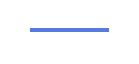
\begin{tikzpicture}[baseline=-0.5ex]
\draw[line width=1.6pt,draw=PrimaryBlue!75] (0,0) -- (1.0,0);
\end{tikzpicture}~\textbf{Strong}\quad
\begin{tikzpicture}[baseline=-0.5ex]
\draw[line width=1.0pt,draw=TealGreen!80] (0,0) -- (1.0,0);
\end{tikzpicture}~\textbf{Moderate}\quad
\begin{tikzpicture}[baseline=-0.5ex]
\draw[line width=0.7pt,dashed,draw=gray!55] (0,0) -- (1.0,0);
\end{tikzpicture}~\textbf{Weak}
\end{center}

\textbf{Fair comparison note:} The PHOENIX system processes the same numerical edge weights shown here. The diagram is a human-readable rendering of identical data; no additional information is available to you vs.\ the machine.

\textbf{Response format:} \textbf{Qualtrics Rank Order item.} Drag/rank the predictor labels from the network in order of treatment priority (1 = highest). Select exactly \textbf{3 targets} (these become the input for Part 4 BFS sub-predictor selection).

\textbf{Time:} Approximately 3.5 minutes per case ($\approx$7 minutes for your two cases).
\end{tcolorbox}

\vspace{0.5em}

% ── C01 Part 3 ───────────────────────────────────────────────────────────────
\subsubsection*{Case C01 --- Part 3}
\dlnote{HCP-PRE-01}

\begin{complaintbox}[title=Case C01 --- 28-year-old software developer]
\small Sleep onset insomnia, bedtime cognitive hyperarousal, social anhedonia, musculoskeletal tension. Duration: 2 months.
\end{complaintbox}

\begin{tcolorbox}[colback=SoftBG,colframe=BorderGrey,boxrule=0.5pt,arc=1.5mm,left=6pt,right=6pt,top=5pt,bottom=5pt]
\small\textbf{21-day monitoring summary:} Screen time past 10\,PM: 16/21 evenings (avg 78 min). Task incompletion: avg 6.2 items/day. Social events: 2.1/week (enjoyment 2.3/10). Pre-sleep offloading used: 3/21 evenings. Physical activity: avg 0.7 sessions/week.
\end{tcolorbox}

\begin{center}
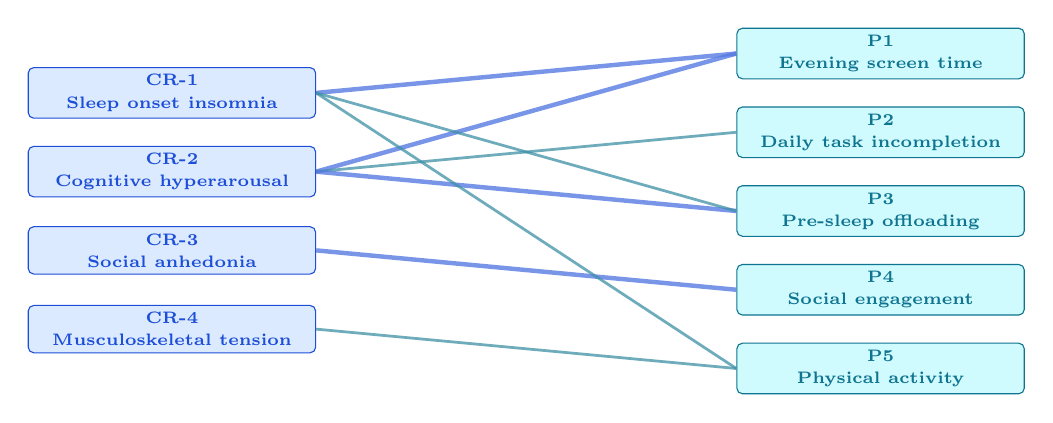
\begin{tikzpicture}[node distance=0pt]
  % Criteria nodes
  \node[crnode] (cr1) at (0, 1.5) {CR-1\\Sleep onset insomnia};
  \node[crnode] (cr2) at (0, 0.5) {CR-2\\Cognitive hyperarousal};
  \node[crnode] (cr3) at (0,-0.5) {CR-3\\Social anhedonia};
  \node[crnode] (cr4) at (0,-1.5) {CR-4\\Musculoskeletal tension};
  % Predictor nodes
  \node[prnode] (p1) at (9, 2.0) {P1\\Evening screen time};
  \node[prnode] (p2) at (9, 1.0) {P2\\Daily task incompletion};
  \node[prnode] (p3) at (9, 0.0) {P3\\Pre-sleep offloading};
  \node[prnode] (p4) at (9,-1.0) {P4\\Social engagement};
  \node[prnode] (p5) at (9,-2.0) {P5\\Physical activity};
  % Edges
  \draw[edgeS] (cr1.east) -- (p1.west);
  \draw[edgeS] (cr2.east) -- (p1.west);
  \draw[edgeM] (cr2.east) -- (p2.west);
  \draw[edgeS] (cr2.east) -- (p3.west);
  \draw[edgeM] (cr1.east) -- (p3.west);
  \draw[edgeS] (cr3.east) -- (p4.west);
  \draw[edgeM] (cr1.east) -- (p5.west);
  \draw[edgeM] (cr4.east) -- (p5.west);
\end{tikzpicture}
\end{center}

\rankresponse{Rank the predictors above in order of treatment priority (1 = highest). Select 2--4 targets only.}

\vspace{0.4em}

% ── C02 Part 3 ───────────────────────────────────────────────────────────────
\subsubsection*{Case C02 --- Part 3}
\dlnote{HCP-PRE-01}

\begin{complaintbox}[title=Case C02 --- 34-year-old healthcare administrator]
\small Recurrent panic episodes, anticipatory anxiety, situational avoidance, occupational impact. Duration: 3 months.
\end{complaintbox}

\begin{tcolorbox}[colback=SoftBG,colframe=BorderGrey,boxrule=0.5pt,arc=1.5mm,left=6pt,right=6pt,top=5pt,bottom=5pt]
\small\textbf{21-day monitoring summary:} Panic episodes: avg 2.3/week. Avoidance events: avg 4.1/day. Safety behaviours: avg 8.7/day. Planned exposures: avg 0.3/day. Work attendance: 60\%. Anticipated anxiety in public settings: 7.8/10.
\end{tcolorbox}

\begin{center}
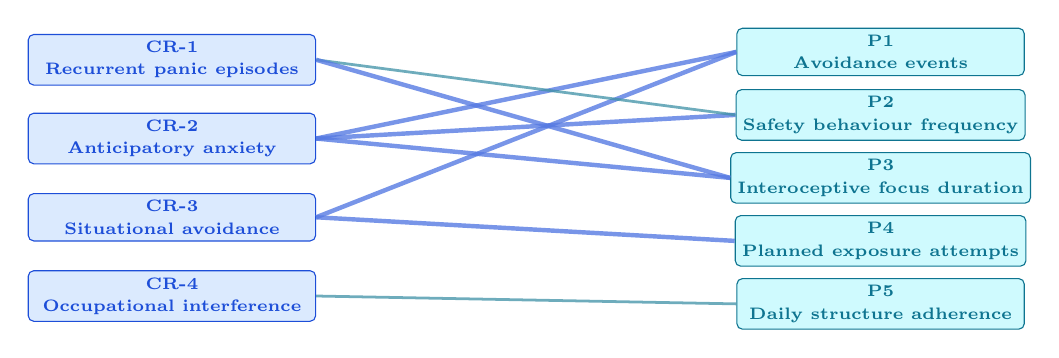
\begin{tikzpicture}[node distance=0pt]
  \node[crnode] (cr1) at (0, 1.5) {CR-1\\Recurrent panic episodes};
  \node[crnode] (cr2) at (0, 0.5) {CR-2\\Anticipatory anxiety};
  \node[crnode] (cr3) at (0,-0.5) {CR-3\\Situational avoidance};
  \node[crnode] (cr4) at (0,-1.5) {CR-4\\Occupational interference};
  \node[prnode] (p1) at (9, 1.6) {P1\\Avoidance events};
  \node[prnode] (p2) at (9, 0.8) {P2\\Safety behaviour frequency};
  \node[prnode] (p3) at (9, 0.0) {P3\\Interoceptive focus duration};
  \node[prnode] (p4) at (9,-0.8) {P4\\Planned exposure attempts};
  \node[prnode] (p5) at (9,-1.6) {P5\\Daily structure adherence};
  \draw[edgeS] (cr3.east) -- (p1.west);
  \draw[edgeS] (cr2.east) -- (p1.west);
  \draw[edgeS] (cr2.east) -- (p2.west);
  \draw[edgeM] (cr1.east) -- (p2.west);
  \draw[edgeS] (cr2.east) -- (p3.west);
  \draw[edgeS] (cr1.east) -- (p3.west);
  \draw[edgeS] (cr3.east) -- (p4.west);
  \draw[edgeM] (cr4.east) -- (p5.west);
\end{tikzpicture}
\end{center}

\rankresponse{Rank the predictors above in order of treatment priority (1 = highest). Select 2--4 targets only.}

\vspace{0.4em}

% ── C03 Part 3 ───────────────────────────────────────────────────────────────
\subsubsection*{Case C03 --- Part 3}
\dlnote{HCP-PRE-02}

\begin{complaintbox}[title=Case C03 --- 41-year-old secondary school teacher]
\small Emotional exhaustion, professional depersonalization, social withdrawal, occupational cognitive difficulties. Duration: 7 months.
\end{complaintbox}

\begin{tcolorbox}[colback=SoftBG,colframe=BorderGrey,boxrule=0.5pt,arc=1.5mm,left=6pt,right=6pt,top=5pt,bottom=5pt]
\small\textbf{21-day monitoring summary:} Evening work violations: avg 5.4/day. Recovery activities: avg 1.2 events/week. Social contacts initiated: avg 0.7/week. Professional mastery moments: avg 0.9/day. Sleep quality: avg 4.1/10.
\end{tcolorbox}

\begin{center}
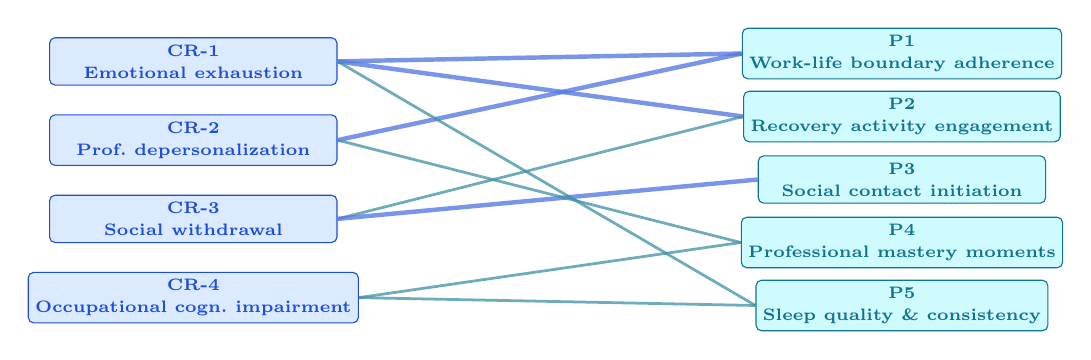
\begin{tikzpicture}[node distance=0pt]
  \node[crnode] (cr1) at (0, 1.5) {CR-1\\Emotional exhaustion};
  \node[crnode] (cr2) at (0, 0.5) {CR-2\\Prof.\ depersonalization};
  \node[crnode] (cr3) at (0,-0.5) {CR-3\\Social withdrawal};
  \node[crnode] (cr4) at (0,-1.5) {CR-4\\Occupational cogn.\ impairment};
  \node[prnode] (p1) at (9, 1.6) {P1\\Work-life boundary adherence};
  \node[prnode] (p2) at (9, 0.8) {P2\\Recovery activity engagement};
  \node[prnode] (p3) at (9, 0.0) {P3\\Social contact initiation};
  \node[prnode] (p4) at (9,-0.8) {P4\\Professional mastery moments};
  \node[prnode] (p5) at (9,-1.6) {P5\\Sleep quality \& consistency};
  \draw[edgeS] (cr1.east) -- (p1.west);
  \draw[edgeS] (cr2.east) -- (p1.west);
  \draw[edgeS] (cr1.east) -- (p2.west);
  \draw[edgeM] (cr3.east) -- (p2.west);
  \draw[edgeS] (cr3.east) -- (p3.west);
  \draw[edgeM] (cr2.east) -- (p4.west);
  \draw[edgeM] (cr4.east) -- (p4.west);
  \draw[edgeM] (cr1.east) -- (p5.west);
  \draw[edgeM] (cr4.east) -- (p5.west);
\end{tikzpicture}
\end{center}

\rankresponse{Rank the predictors above in order of treatment priority (1 = highest). Select 2--4 targets only.}

\vspace{0.4em}

% ── C04 Part 3 ───────────────────────────────────────────────────────────────
\subsubsection*{Case C04 --- Part 3}
\dlnote{HCP-PRE-02}

\begin{complaintbox}[title=Case C04 --- 63-year-old retired professional]
\small Prolonged grief response, sleep maintenance insomnia, guilt-based rumination, absent future orientation. Duration: 9 months post-bereavement.
\end{complaintbox}

\begin{tcolorbox}[colback=SoftBG,colframe=BorderGrey,boxrule=0.5pt,arc=1.5mm,left=6pt,right=6pt,top=5pt,bottom=5pt]
\small\textbf{21-day monitoring summary:} Grief intrusion events: avg 4.2/day. Sleep quality: avg 2.8/10. Social contacts: avg 3.1/week. Guilt thoughts: avg 5.8/day. Future-plan activities: avg 0.4/week. Meaning-making activity: 4/21 days.
\end{tcolorbox}

\begin{center}
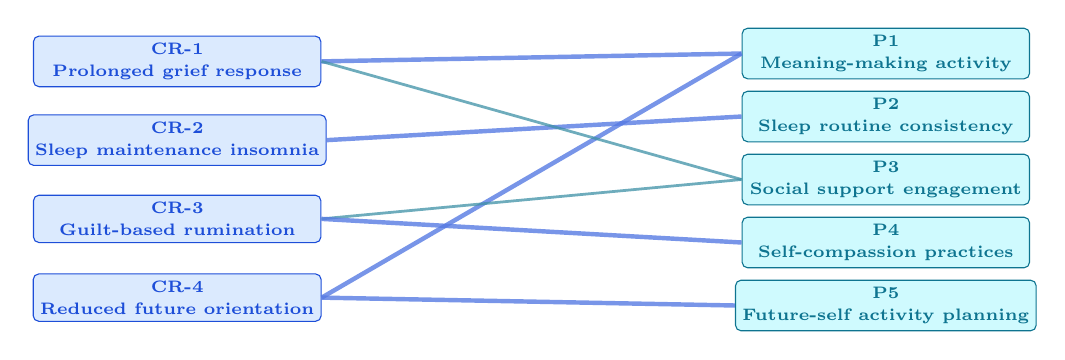
\begin{tikzpicture}[node distance=0pt]
  \node[crnode] (cr1) at (0, 1.5) {CR-1\\Prolonged grief response};
  \node[crnode] (cr2) at (0, 0.5) {CR-2\\Sleep maintenance insomnia};
  \node[crnode] (cr3) at (0,-0.5) {CR-3\\Guilt-based rumination};
  \node[crnode] (cr4) at (0,-1.5) {CR-4\\Reduced future orientation};
  \node[prnode] (p1) at (9, 1.6) {P1\\Meaning-making activity};
  \node[prnode] (p2) at (9, 0.8) {P2\\Sleep routine consistency};
  \node[prnode] (p3) at (9, 0.0) {P3\\Social support engagement};
  \node[prnode] (p4) at (9,-0.8) {P4\\Self-compassion practices};
  \node[prnode] (p5) at (9,-1.6) {P5\\Future-self activity planning};
  \draw[edgeS] (cr1.east) -- (p1.west);
  \draw[edgeS] (cr4.east) -- (p1.west);
  \draw[edgeS] (cr2.east) -- (p2.west);
  \draw[edgeM] (cr1.east) -- (p3.west);
  \draw[edgeM] (cr3.east) -- (p3.west);
  \draw[edgeS] (cr3.east) -- (p4.west);
  \draw[edgeS] (cr4.east) -- (p5.west);
\end{tikzpicture}
\end{center}

\rankresponse{Rank the predictors above in order of treatment priority (1 = highest). Select 2--4 targets only.}

\vspace{0.4em}

% ── C05 Part 3 ───────────────────────────────────────────────────────────────
\subsubsection*{Case C05 --- Part 3}
\dlnote{HCP-PRE-03}

\begin{complaintbox}[title=Case C05 --- 25-year-old postgraduate student]
\small Intrusive harm-related obsessions, compulsive reviewing, harm-trigger avoidance, OCD time interference ($>$2 hr/day). Duration: 20 months.
\end{complaintbox}

\begin{tcolorbox}[colback=SoftBG,colframe=BorderGrey,boxrule=0.5pt,arc=1.5mm,left=6pt,right=6pt,top=5pt,bottom=5pt]
\small\textbf{21-day monitoring summary:} Compulsion/review time: avg 2.4 hrs/day. Avoidance events: avg 3.8/day. Resistance practice: avg 18 min/day. Distress at resisting: 7.2/10. Sleep: avg 5.6 hrs/night. Reassurance seeking: avg 4.1/day.
\end{tcolorbox}

\begin{center}
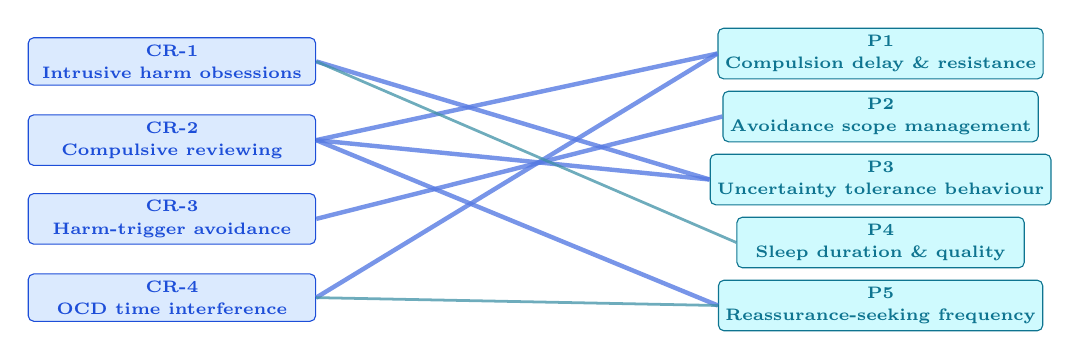
\begin{tikzpicture}[node distance=0pt]
  \node[crnode] (cr1) at (0, 1.5) {CR-1\\Intrusive harm obsessions};
  \node[crnode] (cr2) at (0, 0.5) {CR-2\\Compulsive reviewing};
  \node[crnode] (cr3) at (0,-0.5) {CR-3\\Harm-trigger avoidance};
  \node[crnode] (cr4) at (0,-1.5) {CR-4\\OCD time interference};
  \node[prnode] (p1) at (9, 1.6) {P1\\Compulsion delay \& resistance};
  \node[prnode] (p2) at (9, 0.8) {P2\\Avoidance scope management};
  \node[prnode] (p3) at (9, 0.0) {P3\\Uncertainty tolerance behaviour};
  \node[prnode] (p4) at (9,-0.8) {P4\\Sleep duration \& quality};
  \node[prnode] (p5) at (9,-1.6) {P5\\Reassurance-seeking frequency};
  \draw[edgeS] (cr2.east) -- (p1.west);
  \draw[edgeS] (cr4.east) -- (p1.west);
  \draw[edgeS] (cr3.east) -- (p2.west);
  \draw[edgeS] (cr1.east) -- (p3.west);
  \draw[edgeS] (cr2.east) -- (p3.west);
  \draw[edgeM] (cr1.east) -- (p4.west);
  \draw[edgeS] (cr2.east) -- (p5.west);
  \draw[edgeM] (cr4.east) -- (p5.west);
\end{tikzpicture}
\end{center}

\rankresponse{Rank the predictors above in order of treatment priority (1 = highest). Select 2--4 targets only.}

\vspace{0.4em}

% ── C06 Part 3 ───────────────────────────────────────────────────────────────
\subsubsection*{Case C06 --- Part 3}
\dlnote{HCP-PRE-03}

\begin{complaintbox}[title=Case C06 --- 32-year-old marketing professional]
\small Professional performance anxiety, post-event rumination, pre-event preparation burden, advancement avoidance. Duration: $>$3 years.
\end{complaintbox}

\begin{tcolorbox}[colback=SoftBG,colframe=BorderGrey,boxrule=0.5pt,arc=1.5mm,left=6pt,right=6pt,top=5pt,bottom=5pt]
\small\textbf{21-day monitoring summary:} Presentations entered: avg 0.9/week. Post-event processing time: avg 68 min/event. Pre-event rehearsal: avg 3.2 hrs/event. Perceived performance vs.\ actual: rated 4.1 vs.\ 6.8/10. Advancement opportunities declined: 3 in past 4 weeks.
\end{tcolorbox}

\begin{center}
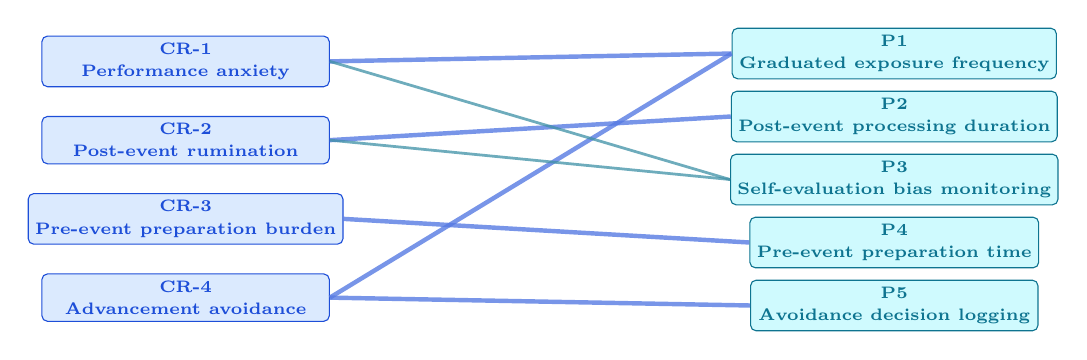
\begin{tikzpicture}[node distance=0pt]
  \node[crnode] (cr1) at (0, 1.5) {CR-1\\Performance anxiety};
  \node[crnode] (cr2) at (0, 0.5) {CR-2\\Post-event rumination};
  \node[crnode] (cr3) at (0,-0.5) {CR-3\\Pre-event preparation burden};
  \node[crnode] (cr4) at (0,-1.5) {CR-4\\Advancement avoidance};
  \node[prnode] (p1) at (9, 1.6) {P1\\Graduated exposure frequency};
  \node[prnode] (p2) at (9, 0.8) {P2\\Post-event processing duration};
  \node[prnode] (p3) at (9, 0.0) {P3\\Self-evaluation bias monitoring};
  \node[prnode] (p4) at (9,-0.8) {P4\\Pre-event preparation time};
  \node[prnode] (p5) at (9,-1.6) {P5\\Avoidance decision logging};
  \draw[edgeS] (cr1.east) -- (p1.west);
  \draw[edgeS] (cr4.east) -- (p1.west);
  \draw[edgeS] (cr2.east) -- (p2.west);
  \draw[edgeM] (cr1.east) -- (p3.west);
  \draw[edgeM] (cr2.east) -- (p3.west);
  \draw[edgeS] (cr3.east) -- (p4.west);
  \draw[edgeS] (cr4.east) -- (p5.west);
\end{tikzpicture}
\end{center}

\rankresponse{Rank the predictors above in order of treatment priority (1 = highest). Select 2--4 targets only.}

\vspace{0.4em}

% ── C07 Part 3 ───────────────────────────────────────────────────────────────
\subsubsection*{Case C07 --- Part 3}
\dlnote{HCP-PRE-04}

\begin{complaintbox}[title=Case C07 --- 46-year-old accounts manager]
\small Persistent low mood and anhedonia, anergia, social isolation, hopelessness. Duration: 14 months.
\end{complaintbox}

\begin{tcolorbox}[colback=SoftBG,colframe=BorderGrey,boxrule=0.5pt,arc=1.5mm,left=6pt,right=6pt,top=5pt,bottom=5pt]
\small\textbf{21-day monitoring summary:} Activity completion rate: 28\%. Social contacts/week: avg 0.8. Mood rated: avg 2.9/10. Sleep wake-time variance: avg $\pm$2.3 hrs. Pleasurable activities: avg 0.9/day. Hopelessness challenge used: avg 0.6/day.
\end{tcolorbox}

\begin{center}
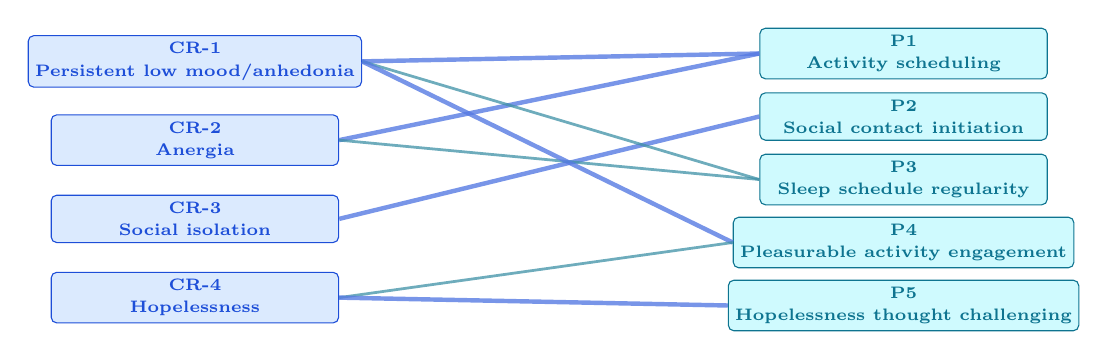
\begin{tikzpicture}[node distance=0pt]
  \node[crnode] (cr1) at (0, 1.5) {CR-1\\Persistent low mood/anhedonia};
  \node[crnode] (cr2) at (0, 0.5) {CR-2\\Anergia};
  \node[crnode] (cr3) at (0,-0.5) {CR-3\\Social isolation};
  \node[crnode] (cr4) at (0,-1.5) {CR-4\\Hopelessness};
  \node[prnode] (p1) at (9, 1.6) {P1\\Activity scheduling};
  \node[prnode] (p2) at (9, 0.8) {P2\\Social contact initiation};
  \node[prnode] (p3) at (9, 0.0) {P3\\Sleep schedule regularity};
  \node[prnode] (p4) at (9,-0.8) {P4\\Pleasurable activity engagement};
  \node[prnode] (p5) at (9,-1.6) {P5\\Hopelessness thought challenging};
  \draw[edgeS] (cr1.east) -- (p1.west);
  \draw[edgeS] (cr2.east) -- (p1.west);
  \draw[edgeS] (cr3.east) -- (p2.west);
  \draw[edgeM] (cr1.east) -- (p3.west);
  \draw[edgeM] (cr2.east) -- (p3.west);
  \draw[edgeS] (cr1.east) -- (p4.west);
  \draw[edgeM] (cr4.east) -- (p4.west);
  \draw[edgeS] (cr4.east) -- (p5.west);
\end{tikzpicture}
\end{center}

\rankresponse{Rank the predictors above in order of treatment priority (1 = highest). Select 2--4 targets only.}

\vspace{0.4em}

% ── C08 Part 3 ───────────────────────────────────────────────────────────────
\subsubsection*{Case C08 --- Part 3}
\dlnote{HCP-PRE-04}

\begin{complaintbox}[title=Case C08 --- 38-year-old project manager]
\small Sustained attention deficit, planning failures, interpersonal inattentiveness, performance shame. Duration: childhood onset.
\end{complaintbox}

\begin{tcolorbox}[colback=SoftBG,colframe=BorderGrey,boxrule=0.5pt,arc=1.5mm,left=6pt,right=6pt,top=5pt,bottom=5pt]
\small\textbf{21-day monitoring summary:} Tasks initiated vs.\ completed: 68\% vs.\ 29\%. Missed commitments: avg 2.1/week. Partner conflict events: avg 4.7/week. External tool use: avg 1.8 uses/day. Positive self-acknowledgment: avg 0.4/day.
\end{tcolorbox}

\begin{center}
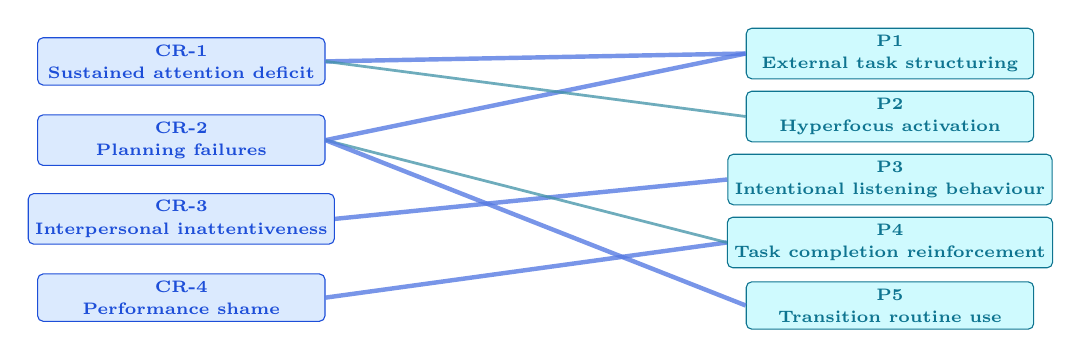
\begin{tikzpicture}[node distance=0pt]
  \node[crnode] (cr1) at (0, 1.5) {CR-1\\Sustained attention deficit};
  \node[crnode] (cr2) at (0, 0.5) {CR-2\\Planning failures};
  \node[crnode] (cr3) at (0,-0.5) {CR-3\\Interpersonal inattentiveness};
  \node[crnode] (cr4) at (0,-1.5) {CR-4\\Performance shame};
  \node[prnode] (p1) at (9, 1.6) {P1\\External task structuring};
  \node[prnode] (p2) at (9, 0.8) {P2\\Hyperfocus activation};
  \node[prnode] (p3) at (9, 0.0) {P3\\Intentional listening behaviour};
  \node[prnode] (p4) at (9,-0.8) {P4\\Task completion reinforcement};
  \node[prnode] (p5) at (9,-1.6) {P5\\Transition routine use};
  \draw[edgeS] (cr2.east) -- (p1.west);
  \draw[edgeS] (cr1.east) -- (p1.west);
  \draw[edgeM] (cr1.east) -- (p2.west);
  \draw[edgeS] (cr3.east) -- (p3.west);
  \draw[edgeS] (cr4.east) -- (p4.west);
  \draw[edgeM] (cr2.east) -- (p4.west);
  \draw[edgeS] (cr2.east) -- (p5.west);
\end{tikzpicture}
\end{center}

\rankresponse{Rank the predictors above in order of treatment priority (1 = highest). Select 2--4 targets only.}

\vspace{0.4em}

% ── C09 Part 3 ───────────────────────────────────────────────────────────────
\subsubsection*{Case C09 --- Part 3}
\dlnote{HCP-PRE-05}

\begin{complaintbox}[title=Case C09 --- 27-year-old sales representative]
\small Intra-day mood cycling, emotional reactivity to rejection, impulsive behaviour, relationship instability. Duration: 3 years.
\end{complaintbox}

\begin{tcolorbox}[colback=SoftBG,colframe=BorderGrey,boxrule=0.5pt,arc=1.5mm,left=6pt,right=6pt,top=5pt,bottom=5pt]
\small\textbf{21-day monitoring summary:} Daily mood range: avg 5.8/10-point scale. ER skill use: avg 1.2/day. Impulsive actions: avg 2.1/day. Interpersonal conflicts: avg 3.8/week. Rejection events perceived: avg 2.4/day. Reappraisal before reacting: avg 0.7/day.
\end{tcolorbox}

\begin{center}
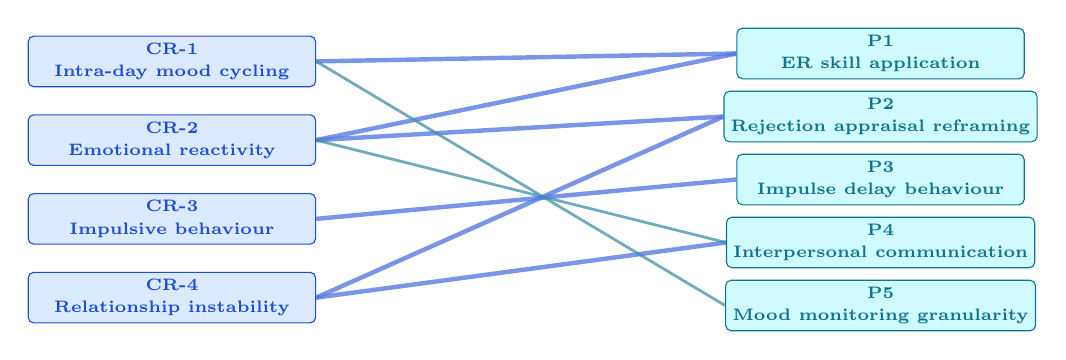
\begin{tikzpicture}[node distance=0pt]
  \node[crnode] (cr1) at (0, 1.5) {CR-1\\Intra-day mood cycling};
  \node[crnode] (cr2) at (0, 0.5) {CR-2\\Emotional reactivity};
  \node[crnode] (cr3) at (0,-0.5) {CR-3\\Impulsive behaviour};
  \node[crnode] (cr4) at (0,-1.5) {CR-4\\Relationship instability};
  \node[prnode] (p1) at (9, 1.6) {P1\\ER skill application};
  \node[prnode] (p2) at (9, 0.8) {P2\\Rejection appraisal reframing};
  \node[prnode] (p3) at (9, 0.0) {P3\\Impulse delay behaviour};
  \node[prnode] (p4) at (9,-0.8) {P4\\Interpersonal communication};
  \node[prnode] (p5) at (9,-1.6) {P5\\Mood monitoring granularity};
  \draw[edgeS] (cr1.east) -- (p1.west);
  \draw[edgeS] (cr2.east) -- (p1.west);
  \draw[edgeS] (cr2.east) -- (p2.west);
  \draw[edgeS] (cr4.east) -- (p2.west);
  \draw[edgeS] (cr3.east) -- (p3.west);
  \draw[edgeS] (cr4.east) -- (p4.west);
  \draw[edgeM] (cr2.east) -- (p4.west);
  \draw[edgeM] (cr1.east) -- (p5.west);
\end{tikzpicture}
\end{center}

\rankresponse{Rank the predictors above in order of treatment priority (1 = highest). Select 2--4 targets only.}

\vspace{0.4em}

% ── C10 Part 3 ───────────────────────────────────────────────────────────────
\subsubsection*{Case C10 --- Part 3}
\dlnote{HCP-PRE-05}

\begin{complaintbox}[title=Case C10 --- 52-year-old operations director]
\small Chronic occupational stress, sleep maintenance insomnia, somatic stress expression, evening alcohol use as coping. Duration: 9 months.
\end{complaintbox}

\begin{tcolorbox}[colback=SoftBG,colframe=BorderGrey,boxrule=0.5pt,arc=1.5mm,left=6pt,right=6pt,top=5pt,bottom=5pt]
\small\textbf{21-day monitoring summary:} Work-related thoughts after 8\,PM: avg 3.4 hrs. Alcohol units: avg 3.1/evening. Headache days: 16/21. Sleep efficiency: avg 62\%. Daytime stress regulation: avg 0.9 events/day. Physical activity: avg 0.4 sessions/week.
\end{tcolorbox}

\begin{center}
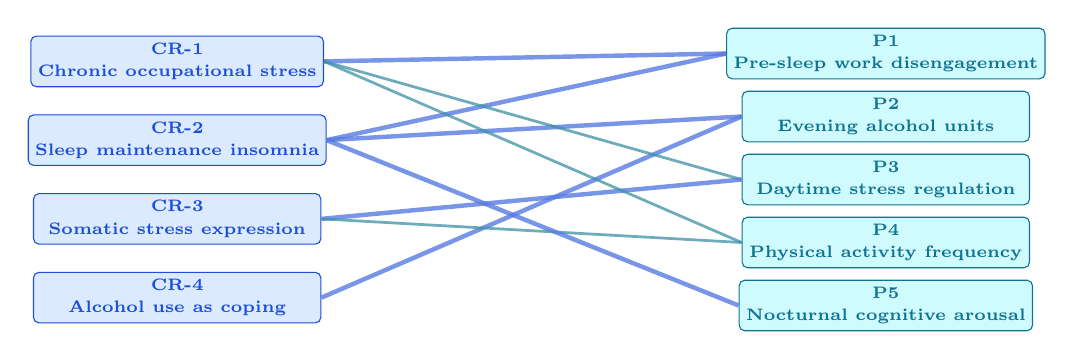
\begin{tikzpicture}[node distance=0pt]
  \node[crnode] (cr1) at (0, 1.5) {CR-1\\Chronic occupational stress};
  \node[crnode] (cr2) at (0, 0.5) {CR-2\\Sleep maintenance insomnia};
  \node[crnode] (cr3) at (0,-0.5) {CR-3\\Somatic stress expression};
  \node[crnode] (cr4) at (0,-1.5) {CR-4\\Alcohol use as coping};
  \node[prnode] (p1) at (9, 1.6) {P1\\Pre-sleep work disengagement};
  \node[prnode] (p2) at (9, 0.8) {P2\\Evening alcohol units};
  \node[prnode] (p3) at (9, 0.0) {P3\\Daytime stress regulation};
  \node[prnode] (p4) at (9,-0.8) {P4\\Physical activity frequency};
  \node[prnode] (p5) at (9,-1.6) {P5\\Nocturnal cognitive arousal};
  \draw[edgeS] (cr2.east) -- (p1.west);
  \draw[edgeS] (cr1.east) -- (p1.west);
  \draw[edgeS] (cr4.east) -- (p2.west);
  \draw[edgeS] (cr2.east) -- (p2.west);
  \draw[edgeM] (cr1.east) -- (p3.west);
  \draw[edgeS] (cr3.east) -- (p3.west);
  \draw[edgeM] (cr1.east) -- (p4.west);
  \draw[edgeM] (cr3.east) -- (p4.west);
  \draw[edgeS] (cr2.east) -- (p5.west);
\end{tikzpicture}
\end{center}

\rankresponse{Rank the predictors above in order of treatment priority (1 = highest). Select 2--4 targets only.}


\newpage

% ─────────────────────────────────────────────────────────────────────────────
\section{Part 4: Updated Observation Model}
% ─────────────────────────────────────────────────────────────────────────────

\begin{tcolorbox}[colback=PartFourBG,colframe=RichPurple,arc=2.5mm,boxrule=0.9pt,left=10pt,right=10pt,top=9pt,bottom=9pt]
\textbf{\color{RichPurple}Part 4 Instructions}

\smallskip
\textbf{Task:} For each case, \textbf{select exactly 6 sub-predictor items} from a list of 20 candidate EMA items, using a \textbf{Breadth-First Selection (BFS)} strategy: choose exactly \textbf{2 sub-predictors per treatment target}, for each of the 3 targets identified in Part 3.

\textbf{Definition --- Sub-predictor:} A \textbf{specific, daily-measurable EMA operationalization} of a treatment target. Where a treatment target is a broad behavioural goal (e.g., ``evening screen time reduction''), the sub-predictors are the concrete daily items that capture it (e.g., \texttt{smartphone use after 22:00 (min)} + \texttt{screen-free interval before sleep (min)}).

\textbf{All 20 candidate items are predictor-type EMA items} --- modifiable behavioural or process variables. None are symptom dimensions or outcome measures. The list contains 6 correct sub-predictors (2 per target) embedded among 14 plausible distractors of similar clinical domain.

\textbf{Selection criteria for each sub-predictor pair:}
\begin{itemize}[topsep=3pt,itemsep=2pt]
\item \textbf{Specificity:} operationalizes the treatment target precisely and without ambiguity
\item \textbf{EMA feasibility:} daily self-reportable in $<$30 seconds (yes/no, count, or minutes)
\item \textbf{Complementarity:} the two selected items capture different facets of the same target (avoid selecting two items that measure the same behaviour)
\end{itemize}

\textbf{Response format:} \textbf{Multiple Choice, select exactly 6} items from the list of 20. The format allows direct comparison with the PHOENIX BFS algorithm output, which selects the same 6 items via a graph-theoretic breadth-first traversal of the bipartite network.

\textbf{Context provided:} Standardised top-3 treatment targets (from Step 03 reference run) appear for each case.

\textbf{Time:} Approximately 3 minutes per case ($\approx$6 minutes for your two cases).
\end{tcolorbox}

\vspace{0.5em}

% ── C01 Part 4 ───────────────────────────────────────────────────────────────
\subsubsection*{Case C01 --- Part 4}
\dlnote{HCP-PRE-01}

\begin{contextbox}
\small\textbf{Standardised top treatment targets (from Step 03 reference run):}
\begin{enumerate}[topsep=2pt,itemsep=1pt,label=\arabic*.]
\item Evening screen time duration (\textit{highest impact on CR-1 and CR-2; data shows consistent late-night use})
\item Pre-sleep cognitive offloading practice (\textit{near-zero usage despite high task backlog; direct CR-2 pathway})
\item Aerobic physical activity (\textit{very low frequency; connects to both CR-1 and CR-4})
\end{enumerate}
\end{contextbox}

\checkboxresponse{Select 2--4 predictors to retain in the next monitoring cycle. Tick each from the list above. Optional: add a 1-sentence operationalization note per selected predictor if a measurement adjustment is needed.}

\vspace{0.4em}

% ── C02 Part 4 ───────────────────────────────────────────────────────────────
\subsubsection*{Case C02 --- Part 4}
\dlnote{HCP-PRE-01}

\begin{contextbox}
\small\textbf{Standardised top treatment targets:}
\begin{enumerate}[topsep=2pt,itemsep=1pt,label=\arabic*.]
\item Planned exposure attempts (\textit{nearly absent in monitoring data; direct avoidance reduction pathway})
\item Safety behaviour frequency (\textit{high frequency sustaining anticipatory anxiety; key maintenance loop})
\item Interoceptive focus duration (\textit{elevated; fuels panic escalation cycle})
\end{enumerate}
\end{contextbox}

\checkboxresponse{Select 2--4 predictors to retain in the next monitoring cycle. Tick each from the list above. Optional: add a 1-sentence operationalization note per selected predictor if a measurement adjustment is needed.}

\vspace{0.4em}

% ── C03 Part 4 ───────────────────────────────────────────────────────────────
\subsubsection*{Case C03 --- Part 4}
\dlnote{HCP-PRE-02}

\begin{contextbox}
\small\textbf{Standardised top treatment targets:}
\begin{enumerate}[topsep=2pt,itemsep=1pt,label=\arabic*.]
\item Work-life boundary adherence (\textit{highest maintenance factor for exhaustion; avg 5.4 violations/day})
\item Recovery activity engagement (\textit{critical low at 1.2 events/week; addresses CR-1 and CR-3})
\item Professional mastery moments (\textit{addresses depersonalization; low but showing variability})
\end{enumerate}
\end{contextbox}

\checkboxresponse{Select 2--4 predictors to retain in the next monitoring cycle. Tick each from the list above. Optional: add a 1-sentence operationalization note per selected predictor if a measurement adjustment is needed.}

\vspace{0.4em}

% ── C04 Part 4 ───────────────────────────────────────────────────────────────
\subsubsection*{Case C04 --- Part 4}
\dlnote{HCP-PRE-02}

\begin{contextbox}
\small\textbf{Standardised top treatment targets:}
\begin{enumerate}[topsep=2pt,itemsep=1pt,label=\arabic*.]
\item Structured meaning-making activity (\textit{used only 4/21 days; high potential for CR-1 and CR-4})
\item Sleep routine consistency (\textit{poor sleep quality; downstream effects on grief processing})
\item Self-compassion practices (\textit{guilt ruminative burden high; underused coping resource})
\end{enumerate}
\end{contextbox}

\checkboxresponse{Select 2--4 predictors to retain in the next monitoring cycle. Tick each from the list above. Optional: add a 1-sentence operationalization note per selected predictor if a measurement adjustment is needed.}

\vspace{0.4em}

% ── C05 Part 4 ───────────────────────────────────────────────────────────────
\subsubsection*{Case C05 --- Part 4}
\dlnote{HCP-PRE-03}

\begin{contextbox}
\small\textbf{Standardised top treatment targets:}
\begin{enumerate}[topsep=2pt,itemsep=1pt,label=\arabic*.]
\item Compulsion delay and resistance practice (\textit{used minimally; avg 18 min vs target 60+; core ERP component})
\item Avoidance scope management (\textit{high avoidance events maintain the obsessional cycle})
\item Uncertainty tolerance behaviour (\textit{low; drives both intrusions and reviewing})
\end{enumerate}
\end{contextbox}

\checkboxresponse{Select 2--4 predictors to retain in the next monitoring cycle. Tick each from the list above. Optional: add a 1-sentence operationalization note per selected predictor if a measurement adjustment is needed.}

\vspace{0.4em}

% ── C06 Part 4 ───────────────────────────────────────────────────────────────
\subsubsection*{Case C06 --- Part 4}
\dlnote{HCP-PRE-03}

\begin{contextbox}
\small\textbf{Standardised top treatment targets:}
\begin{enumerate}[topsep=2pt,itemsep=1pt,label=\arabic*.]
\item Graduated professional exposure frequency (\textit{low frequency; key mechanism for anxiety reduction})
\item Post-event processing duration (\textit{avg 87 min/event; major maintenance factor for CR-2})
\item Avoidance decision logging (\textit{avg 1.4 opportunities declined/week; directly limits advancement})
\end{enumerate}
\end{contextbox}

\checkboxresponse{Select 2--4 predictors to retain in the next monitoring cycle. Tick each from the list above. Optional: add a 1-sentence operationalization note per selected predictor if a measurement adjustment is needed.}

\vspace{0.4em}

% ── C07 Part 4 ───────────────────────────────────────────────────────────────
\subsubsection*{Case C07 --- Part 4}
\dlnote{HCP-PRE-04}

\begin{contextbox}
\small\textbf{Standardised top treatment targets:}
\begin{enumerate}[topsep=2pt,itemsep=1pt,label=\arabic*.]
\item Daily activity scheduling and completion (\textit{completion rate 28\%; behavioral activation core mechanism})
\item Sleep schedule regularity (\textit{$\pm$2.3 hr variance; disrupts mood and energy regulation})
\item Social contact initiation (\textit{avg 0.8/week; critical for CR-3 and indirect mood lifting})
\end{enumerate}
\end{contextbox}

\checkboxresponse{Select 2--4 predictors to retain in the next monitoring cycle. Tick each from the list above. Optional: add a 1-sentence operationalization note per selected predictor if a measurement adjustment is needed.}

\vspace{0.4em}

% ── C08 Part 4 ───────────────────────────────────────────────────────────────
\subsubsection*{Case C08 --- Part 4}
\dlnote{HCP-PRE-04}

\begin{contextbox}
\small\textbf{Standardised top treatment targets:}
\begin{enumerate}[topsep=2pt,itemsep=1pt,label=\arabic*.]
\item External task structuring tool use (\textit{inconsistent at 1.8 uses/day; core scaffolding system})
\item Intentional listening behaviour (\textit{partner conflict avg 4.7/week; direct CR-3 pathway})
\item Task completion reinforcement (\textit{very low; shame cycle maintenance factor})
\end{enumerate}
\end{contextbox}

\checkboxresponse{Select 2--4 predictors to retain in the next monitoring cycle. Tick each from the list above. Optional: add a 1-sentence operationalization note per selected predictor if a measurement adjustment is needed.}

\vspace{0.4em}

% ── C09 Part 4 ───────────────────────────────────────────────────────────────
\subsubsection*{Case C09 --- Part 4}
\dlnote{HCP-PRE-05}

\begin{contextbox}
\small\textbf{Standardised top treatment targets:}
\begin{enumerate}[topsep=2pt,itemsep=1pt,label=\arabic*.]
\item Emotion regulation skill application (\textit{low use; mood range 5.8 pts/day; primary intervention lever})
\item Impulse delay behaviour (\textit{avg 2.1 impulsive actions/day; core target for CR-3 and CR-4})
\item Rejection appraisal reframing (\textit{avg 0.7/day despite 2.4 perceived rejection events/day})
\end{enumerate}
\end{contextbox}

\checkboxresponse{Select 2--4 predictors to retain in the next monitoring cycle. Tick each from the list above. Optional: add a 1-sentence operationalization note per selected predictor if a measurement adjustment is needed.}

\vspace{0.4em}

% ── C10 Part 4 ───────────────────────────────────────────────────────────────
\subsubsection*{Case C10 --- Part 4}
\dlnote{HCP-PRE-05}

\begin{contextbox}
\small\textbf{Standardised top treatment targets:}
\begin{enumerate}[topsep=2pt,itemsep=1pt,label=\arabic*.]
\item Pre-sleep work disengagement routine (\textit{absent; nocturnal cognitive arousal drives CR-2})
\item Evening alcohol units (\textit{avg 3.1 units; perpetuates insomnia; priority reduction target})
\item Daytime stress regulation behaviour (\textit{avg 0.9 events/day; low but trainable})
\end{enumerate}
\end{contextbox}

\checkboxresponse{Select 2--4 predictors to retain in the next monitoring cycle. Tick each from the list above. Optional: add a 1-sentence operationalization note per selected predictor if a measurement adjustment is needed.}

\newpage

% ─────────────────────────────────────────────────────────────────────────────
\section{Part 5: Tailored Intervention Message}
% ─────────────────────────────────────────────────────────────────────────────

\begin{tcolorbox}[colback=PartFiveBG,colframe=TealGreen,arc=2.5mm,boxrule=0.9pt,left=10pt,right=10pt,top=9pt,bottom=9pt]
\textbf{\color{TealGreen}Part 5 Instructions}

\smallskip
\textbf{Task:} For each case, complete two items: (A) classify the person's \textbf{HAPA motivational phase}, and (B) write a \textbf{brief personalized digital coaching message} targeting the top treatment target.

\textbf{(A) HAPA phase classification} (Health Action Process Approach; Schwarzer, 1992):
\begin{itemize}[topsep=3pt,itemsep=2pt]
\item \textbf{Pre-intentional} --- not yet motivated to change the target behaviour; lacks perceived risk or outcome expectancy. Message focus: risk awareness, outcome expectancy, motivational framing.
\item \textbf{Intentional} --- motivated to change but has not yet formed a concrete action plan; intention--behaviour gap. Message focus: specific goal-setting, implementation intentions (``when--then'' planning), action planning.
\item \textbf{Action/Maintenance} --- already attempting or sustaining behaviour change; vulnerable to lapse. Message focus: coping planning, recovery self-efficacy, relapse prevention, positive reinforcement.
\end{itemize}

\textbf{(B) Message requirements:}
\begin{itemize}[topsep=3pt,itemsep=2pt]
\item \textbf{Length:} 2--4 sentences
\item \textbf{Person:} second person (``you / your'')
\item \textbf{Tone:} warm, empathic, and professionally supportive --- neither clinical/distant nor colloquial
\item \textbf{Content:} address the top treatment target explicitly; include a concrete, actionable step; match the HAPA phase (motivational, planning-oriented, or coping-oriented)
\item \textbf{No jargon:} do not use diagnostic labels, clinical acronyms, or technical EMA/network terminology
\end{itemize}

\textbf{Response format:} Two Qualtrics items per case: (A) multiple choice for HAPA phase, (B) Text Entry (Medium) for message.

\textbf{Context provided:} Top treatment target, primary barrier type, and suggested coping strategy per case.

\textbf{Time:} Approximately 3.5 minutes per case ($\approx$7 minutes for your two cases).
\end{tcolorbox}

\vspace{0.5em}

% ── C01 Part 5 ───────────────────────────────────────────────────────────────
\subsubsection*{Case C01 --- Part 5}

\begin{contextbox}
\small
\textbf{Primary challenge:} Difficulty falling asleep due to an overactive mind at bedtime; social disconnection.\\
\textbf{Top treatment target:} Evening screen time reduction and pre-sleep wind-down routine.\\
\textbf{Main barrier:} \textit{Self-efficacy} --- habitual screen use is experienced as a necessary decompression tool; low confidence that reducing it is possible without losing the relaxation benefit.\\
\textbf{Coping strategy:} Implementation intention with a substitution plan (replace screen time with a brief physical or written offloading activity in the 30 minutes before bed).
\end{contextbox}

\haparesponse{(A) Select the HAPA motivational phase for this person. (B) Write a 2--3 sentence personalized coaching message addressing the top treatment target and coping strategy above.}

\vspace{0.4em}

% ── C02 Part 5 ───────────────────────────────────────────────────────────────
\subsubsection*{Case C02 --- Part 5}

\begin{contextbox}
\small
\textbf{Primary challenge:} Fear of panic episodes leading to increasing avoidance and reduced daily functioning.\\
\textbf{Top treatment target:} Planned exposure --- gradually re-entering feared situations.\\
\textbf{Main barrier:} \textit{Outcome expectancy} --- strong belief that entering avoided situations will inevitably lead to a panic episode that cannot be managed.\\
\textbf{Coping strategy:} Planning a hierarchy of small, manageable exposure steps with a coping script prepared in advance.
\end{contextbox}

\haparesponse{(A) Select the HAPA motivational phase for this person. (B) Write a 2--3 sentence personalized coaching message addressing the top treatment target and coping strategy above.}

\vspace{0.4em}

% ── C03 Part 5 ───────────────────────────────────────────────────────────────
\subsubsection*{Case C03 --- Part 5}

\begin{contextbox}
\small
\textbf{Primary challenge:} Profound occupational exhaustion with loss of meaning and progressive social withdrawal.\\
\textbf{Top treatment target:} Work-life boundary enforcement --- structured protection of non-work time.\\
\textbf{Main barrier:} \textit{Action planning deficit} --- no concrete plan for what a work boundary looks like or when it applies; boundary attempts collapse under work demands.\\
\textbf{Coping strategy:} Implementation intention with a specific boundary signal (e.g., device-off at a set time) paired with one simple recovery activity immediately after.
\end{contextbox}

\haparesponse{(A) Select the HAPA motivational phase for this person. (B) Write a 2--3 sentence personalized coaching message addressing the top treatment target and coping strategy above.}

\vspace{0.4em}

% ── C04 Part 5 ───────────────────────────────────────────────────────────────
\subsubsection*{Case C04 --- Part 5}

\begin{contextbox}
\small
\textbf{Primary challenge:} Prolonged grief with pervasive guilt and absence of forward-looking engagement.\\
\textbf{Top treatment target:} Structured meaning-making activity --- engaging with memory, legacy, or creative activities that honour the loss and rebuild connection to the future.\\
\textbf{Main barrier:} \textit{Motivational deficit} --- absence of motivation or a clear sense of what is worth doing; grief-related anhedonia blocks initiation.\\
\textbf{Coping strategy:} Reducing the size of the first step to a minimal, time-limited activity (e.g., writing one sentence in a memory book once this week).
\end{contextbox}

\haparesponse{(A) Select the HAPA motivational phase for this person. (B) Write a 2--3 sentence personalized coaching message addressing the top treatment target and coping strategy above.}

\vspace{0.4em}

% ── C05 Part 5 ───────────────────────────────────────────────────────────────
\subsubsection*{Case C05 --- Part 5}

\begin{contextbox}
\small
\textbf{Primary challenge:} Distressing intrusive thoughts with extensive compulsive reviewing consuming hours daily.\\
\textbf{Top treatment target:} Compulsion delay and resistance practice --- extending the time between intrusion and reviewing response.\\
\textbf{Main barrier:} \textit{Perceived risk} --- strong overestimation that not reviewing will lead to actual harm; reviewing feels morally necessary even when recognized as irrational.\\
\textbf{Coping strategy:} Delay rule --- committing to a 5-minute pause before any reviewing begins, with a brief mindful grounding exercise during the delay.
\end{contextbox}

\haparesponse{(A) Select the HAPA motivational phase for this person. (B) Write a 2--3 sentence personalized coaching message addressing the top treatment target and coping strategy above.}

\vspace{0.4em}

% ── C06 Part 5 ───────────────────────────────────────────────────────────────
\subsubsection*{Case C06 --- Part 5}

\begin{contextbox}
\small
\textbf{Primary challenge:} Intense anxiety in professional performance situations with extensive post-event rumination.\\
\textbf{Top treatment target:} Graduated professional exposure --- entering and completing professional situations despite anxiety.\\
\textbf{Main barrier:} \textit{Self-efficacy gap} --- strong conviction that performance is objectively poor and that exposure will confirm this; distorted self-evaluation persists despite contradictory external feedback.\\
\textbf{Coping strategy:} Behavioural experiment approach --- after the next professional exposure, record the predicted rating and then gather actual feedback to compare.
\end{contextbox}

\haparesponse{(A) Select the HAPA motivational phase for this person. (B) Write a 2--3 sentence personalized coaching message addressing the top treatment target and coping strategy above.}

\vspace{0.4em}

% ── C07 Part 5 ───────────────────────────────────────────────────────────────
\subsubsection*{Case C07 --- Part 5}

\begin{contextbox}
\small
\textbf{Primary challenge:} Persistent low mood and anergia with near-complete loss of activity and social connection.\\
\textbf{Top treatment target:} Daily activity scheduling and completion --- behavioural activation through planned, minimal daily activities.\\
\textbf{Main barrier:} \textit{Planning barrier} --- no structured activity menu available; activities feel meaningless before attempting them; anergia blocks initiation.\\
\textbf{Coping strategy:} Activity menu strategy --- pre-selecting three very small activities (5 minutes each) the night before, with a ``done-is-enough'' standard.
\end{contextbox}

\haparesponse{(A) Select the HAPA motivational phase for this person. (B) Write a 2--3 sentence personalized coaching message addressing the top treatment target and coping strategy above.}

\vspace{0.4em}

% ── C08 Part 5 ───────────────────────────────────────────────────────────────
\subsubsection*{Case C08 --- Part 5}

\begin{contextbox}
\small
\textbf{Primary challenge:} Executive functioning difficulties creating task failures, relationship strain, and chronic shame.\\
\textbf{Top treatment target:} External task structuring tool use --- consistent daily use of an external system (written or digital) to scaffold task planning and completion.\\
\textbf{Main barrier:} \textit{Habit resistance} --- tools have been tried before but abandoned; low self-efficacy about sustaining system use; shame about needing external scaffolding.\\
\textbf{Coping strategy:} Minimum viable habit --- one non-negotiable daily check-in with the tool (morning review, 3 minutes) as an anchored routine rather than a complex system.
\end{contextbox}

\haparesponse{(A) Select the HAPA motivational phase for this person. (B) Write a 2--3 sentence personalized coaching message addressing the top treatment target and coping strategy above.}

\vspace{0.4em}

% ── C09 Part 5 ───────────────────────────────────────────────────────────────
\subsubsection*{Case C09 --- Part 5}

\begin{contextbox}
\small
\textbf{Primary challenge:} Rapid mood swings and intense emotional reactivity causing impulsive behaviour and relationship breakdown.\\
\textbf{Top treatment target:} Emotion regulation skill application --- consistent use of a specific, rehearsed skill when emotional intensity rises.\\
\textbf{Main barrier:} \textit{Coping self-efficacy} --- strong doubts about ability to manage intense affect; past skill use attempts have felt ineffective in the moment of peak emotion.\\
\textbf{Coping strategy:} Pre-committed cue-action plan --- identifying one specific physical cue of rising emotion and linking it to one specific skill (e.g., TIPP, grounding) rehearsed daily in low-affect moments.
\end{contextbox}

\haparesponse{(A) Select the HAPA motivational phase for this person. (B) Write a 2--3 sentence personalized coaching message addressing the top treatment target and coping strategy above.}

\vspace{0.4em}

% ── C10 Part 5 ───────────────────────────────────────────────────────────────
\subsubsection*{Case C10 --- Part 5}

\begin{contextbox}
\small
\textbf{Primary challenge:} Chronic work stress with fragmented sleep, somatic symptoms, and alcohol as the primary coping mechanism.\\
\textbf{Top treatment target:} Pre-sleep work disengagement routine --- a structured sequence that creates a clear boundary between work and sleep.\\
\textbf{Main barrier:} \textit{Habit strength} --- nightly alcohol use is a deeply established coping pattern perceived as essential for sleep; no alternative wind-down routine currently exists.\\
\textbf{Coping strategy:} Routine substitution --- designing a specific 20-minute wind-down sequence that begins at the same time each evening and replaces (rather than prohibits) alcohol as a cue-to-sleep signal.
\end{contextbox}

\haparesponse{(A) Select the HAPA motivational phase for this person. (B) Write a 2--3 sentence personalized coaching message addressing the top treatment target and coping strategy above.}

\newpage

% ─────────────────────────────────────────────────────────────────────────────
\section{Completion and Submission}
% ─────────────────────────────────────────────────────────────────────────────

Thank you for completing all five parts of this survey. Your responses across the ten cases will form the expert reference corpus for the PHOENIX evaluation study. Before submitting, please review the checklist below.

\begin{instrbox}[title=Pre-submission checklist]
\begin{itemize}
\item[$\square$] I have provided responses for all 10 cases in Part 1 (operationalization).
\item[$\square$] I have provided responses for all 10 cases in Part 2 (initial model).
\item[$\square$] I have provided responses for all 10 cases in Part 3 (treatment targets).
\item[$\square$] I have provided responses for all 10 cases in Part 4 (updated model).
\item[$\square$] I have provided responses for all 10 cases in Part 5 (intervention message).
\item[$\square$] My responses reflect my genuine clinical judgment without external reference.
\item[$\square$] I understand that my responses will be anonymized and used solely for evaluation purposes.
\end{itemize}
\end{instrbox}

\medskip
Once submitted, your responses will be assigned a pseudonymous participant ID and will not be modifiable. If you have any questions or concerns, please contact the researcher at \texttt{stijn.vanseveren@ugent.be} before submitting.

\vspace{0.8em}

\begin{tcolorbox}[colback=AccentBlue,colframe=PrimaryBlue,arc=2mm,boxrule=0.6pt,left=8pt,right=8pt,top=7pt,bottom=7pt]
\small\centering
\textbf{Qualtrics: End of Survey block}\\
Include: automatic acknowledgement message and unique response ID display.\\
Optional: demographic block (professional background, years of clinical experience, primary discipline) for covariate adjustment in the analysis.
\end{tcolorbox}

% ─────────────────────────────────────────────────────────────────────────────
\section{Qualtrics Configuration Notes}
% ─────────────────────────────────────────────────────────────────────────────

\subsection*{Block Structure}

Implement the survey as five sequential Qualtrics \textbf{blocks}, one per part. Configure the following:

\begin{enumerate}
\item \textbf{Block display logic:} Show blocks sequentially (Block 1 must be completed before Block 2 is unlocked). Use Qualtrics \textit{Survey Flow} to enforce order.
\item \textbf{Item type:} All 50 response items are \textit{Text Entry (Essay/Large)} questions. Do not add scale or multiple-choice items within the generation phase.
\item \textbf{Forced response:} Set all 50 items to \textit{Request response} (allow but flag missing). Do not use forced response, as some HCPs may prefer to leave a case blank rather than respond speculatively.
\item \textbf{Progress bar:} Enable the progress bar. Set milestones at Part 1 end (20\%), Part 2 end (40\%), Part 3 end (60\%), Part 4 end (80\%), and submission (100\%).
\item \textbf{Session saving:} Enable \textit{Save and Continue} so participants can complete across multiple sittings.
\item \textbf{Timing:} Enable \textit{Page Timer} on each block for session-length analysis.
\item \textbf{Anonymity:} Disable IP recording if institutional ethics requires anonymous participation; use anonymous survey links.
\item \textbf{Demographic block:} Add an optional final block collecting: (a) professional discipline (psychiatry / clinical psychology / nursing / general practice / other), (b) years of clinical experience, (c) primary patient population (adult, youth, older adult, mixed), (d) familiarity with digital mental health tools (1--5).
\end{enumerate}

\subsection*{Participant ID Assignment}

Assign each participant a random 4-character alphanumeric ID (e.g., \texttt{HCP\_PRE\_A3F7}) at survey start. Display it prominently on the completion page. Record it in the response metadata. This ID is used to link PRE-phase responses to the blinded POST-phase evaluation.

\subsection*{Data Export Format}

Export responses as CSV with one column per item (Part\#\_Case\#) and one row per participant. The column naming convention is: \texttt{P1\_C01}, \texttt{P1\_C02}, \ldots, \texttt{P5\_C10}.

\end{document}
